% !TeX program = xelatex
\documentclass[final,5p,times,twocolumn]{elsarticle/elsarticle}

\usepackage{amsmath, amssymb}
\usepackage{booktabs, multirow, array, longtable}
\usepackage{threeparttable}
\usepackage{tikz}
\usetikzlibrary{positioning, arrows.meta, shapes.geometric, calc, fit, backgrounds, decorations.pathmorphing, shadows}
\usepackage{float}
\usepackage{algorithm}
\usepackage{algorithmic}
\usepackage[colorlinks=true, linkcolor=black, citecolor=black, urlcolor=blue]{hyperref}
\pdfstringdefDisableCommands{\def\corref#1{}}

\graphicspath{{../}}

\renewcommand{\algorithmicrequire}{\textbf{Input:}}
\renewcommand{\algorithmicensure}{\textbf{Output:}}

\journal{Future Generation Computer Systems}

\begin{document}

\begin{frontmatter}

    \title{Trust-Flow-Driven Trusted Federated Learning with TEE-Anchored Admission in Edge Computing}

    \author[inst1]{Jiakai Zhou}
    \ead{w1lsp0@stud.tjut.edu.cn}
    \author[inst1]{Chao Bu\corref{cor1}}
    \ead{bc_0722@163.com}

    \cortext[cor1]{Corresponding author. ORCID: 0000-0001-8990-5487.}

    \affiliation[inst1]{organization={School of Computer Science and Engineering, Tianjin University of Technology},
        city={Tianjin},
        country={China}}

    \begin{abstract}
        Federated learning must distinguish an update produced by an admissible
        execution from an update that is useful and semantically safe under
        Non-IID data. A static trusted-execution gate cannot answer the second
        question, whereas a single update-quality threshold can remove legitimate
        long-tail clients. This paper presents Trust Flow, a system-level
        decision framework that keeps execution credibility, current update
        content, long-term utility, and short-term risk as separate evidence
        streams until aggregation. A TEE-anchored trusted management and
        attestation agent (TMAA) supplies admission evidence; an explicit Kalman
        recursion and a dual-stream Beta/EMA state model define cold-start and
        cross-round behavior; and a layer-wise rule performs risk-dependent
        clipping with data-size-aware survivor re-normalization. The evaluation
        uses two Intel/AMD TEE-capable hardware configurations, Flower/PyTorch,
        CIFAR-10, 20 admitted clients, six concurrent attack behaviors, five
        seeds per platform, and a 30\% malicious setting. Targeted ASR is
        macro-averaged over trigger, clean-label, and semantic attacks, whereas
        untargeted attacks are evaluated through clean accuracy, loss, and state
        transitions. Under the stated protocol, Trust Flow reaches 92.31\%
        clean accuracy, 10.21\% targeted ASR, and no permanent false ban in the
        tested runs.
    \end{abstract}

    \begin{keyword}
        Federated learning \sep Edge computing \sep Trusted execution environment \sep Risk state modeling \sep Layered robust aggregation \sep Backdoor defense
    \end{keyword}

\end{frontmatter}

\section{Introduction}

Current advancements in terminal device computing power enable efficient local model training using on-device data. Meanwhile, to better aggregate multi-device training experiences for collaborative model optimization while preserving local data privacy, the federated learning paradigm has been extensively studied \cite{kairouz2021flsurvey}. Its core feature---exchanging only model parameters without offloading data---is widely applied in distributed collaborative training, serving as a critical pillar for edge intelligence. However, as the interconnected network environment becomes increasingly open, the performance bottlenecks of federated learning no longer reside solely in model architecture or optimizer design. The trustworthiness and robustness of the aggregation phase have emerged as vital factors determining overall availability. In practical scenarios, edge devices often exhibit significant heterogeneity in both data distribution and processing capabilities. Furthermore, fully constraining the behaviors of participating clients remains challenging. Such characteristics inevitably amplify statistical drifts and introduce security risks during empirical aggregation.

In standard federated learning paradigms, clients upload parameters after completing local data processing and model training. The server then aggregates these local updates and distributes the updated global model, iterating this process until convergence. Evidently, this workflow encounters multiple vulnerabilities within the increasingly open, multi-edge interconnected network. Open training environments inherently lack mandatory integrity constraints. Malicious clients can bypass actual training, directly crafting and uploading poisoned parameters, thereby severely impairing the server's ability to verify the authenticity of aggregated updates. Several studies propose methods based on trusted execution or verifiable training \cite{lu2025tmt,zhang2025rppfl,r1_tee_integrity}, employing hardware-assisted remote attestation to ensure local training authenticity. Nevertheless, these mechanisms fail to address scenarios where the training process is genuine but the model updates are injected with malicious features. Furthermore, attackers execute parameter poisoning or stealthy backdoor attacks \cite{bagdasaryan2020backdoor,wang2019neuralcleanse} by embedding malicious triggers within normal update distributions, drastically reducing the success rate of single-round detection. To alleviate the instability of single-round assessments, researchers have introduced methods based on historical reputation and similarity \cite{cao2021fltrust,fung2020foolsgold} that leverage cross-round information. Yet, these approaches suffer from delayed recognition of sleeper attacks, where adversaries accumulate reputation early on before engaging in persistent, low-amplitude poisoning. Additionally, single-reputation scores combined with fixed-threshold mechanisms remain highly inadequate for identifying deep abnormal trigger features.

The presence of non-independent and identically distributed (Non-IID) data across devices increases the directional dispersion of optimal updates. This heterogeneity easily blurs the boundary between normal statistical fluctuations and anomalous deviations, creating a conflict between robustness and generalization under strong Non-IID conditions. Certain approaches rely on distance-based exclusion or statistical truncation to suppress abnormal updates \cite{blanchard2017krum,yin2018byzantine}, while others adaptively adjust weights to mitigate heterogeneous impacts \cite{wang2025rasa}. Under severe long-tail distributions, however, such methods often misclassify legitimately drifted parameter updates as anomalies. This misjudgment can lead to the excessive exclusion of crucial heterogeneous information, significantly degrading the model's generalization capability. In real-world edge intelligence scenarios, these challenges---open execution environments, stealthy cross-round attacks, and pronounced heterogeneous statistical drifts---rarely occur in isolation. Multiple factors frequently compound, leading to intractable dilemmas such as elevated false positive rates from tightening interception thresholds or increased false negative rates when relaxing them. Consequently, establishing a unified state modeling and coordinated decision-making mechanism spanning the entire workflow remains a critical challenge. Such a mechanism must balance client admission and trustworthiness during local training with low false positive and high recall requirements during aggregation, all while maintaining the convergence and generalization performance of collaborative model optimization.

To tackle the three major challenges outlined above, this paper proposes a trusted federated aggregation mechanism driven by a full-process trust flow, conceptualized from a hardware-software co-design perspective. This mechanism follows the execution pipeline of federated learning. During client admission and local training, TEE remote attestation, runtime feature entropy analysis, and Kalman filtering are introduced to formulate a dynamic admission trust score that updates across rounds. At the server auditing stage, the current-round content quality is evaluated based on a pure reference direction. The client's state is then decoupled into a historical utility flow and an instant risk flow, utilizing Bayesian posterior inference and risk EMA to separately characterize long-term contributions and short-term anomalies. During the aggregation phase, layered risk gating, survivor weight re-normalization, and dynamic clipping are executed based on these trust states. This strategy suppresses malicious updates while retaining legitimate heterogeneous contributions, effectively mitigating the tradeoff between security and generalization under Non-IID conditions.

The primary contributions of this paper are system-level and concern the
ordering and interface between established mechanisms rather than a new
cryptographic primitive or Byzantine estimator:
\begin{enumerate}
    \item \textbf{TEE-anchored admission with an explicit cold-start policy.} Remote attestation defines the execution boundary, while entropy-derived observations and a covariance-aware Kalman recursion produce a continuously updated admission score. A newly admitted client starts in NORMAL and cannot be permanently blacklisted in its first round.
    \item \textbf{Dual-stream state evolution.} Explicit decayed Beta updates describe historical utility, while an EMA of the strongest current risk probe preserves short-term attack evidence. The two streams are fused only when aggregation privilege is computed.
    \item \textbf{Risk-gated layered aggregation.} Layer sensitivity scores determine thresholds and clipping radii; the original data-volume weight is retained and only surviving mass is re-normalized.
    \item \textbf{Protocol-matched evaluation.} Two Intel/AMD TEE-capable platforms, five seeds per platform, a shared 5,000-sample client-training pool plus a server-held 500-sample proxy set, a CIFAR-10-adapted ResNet-18, and six concurrent attack behaviors are evaluated. Recent defenses are discussed as positioning references and are not assigned unverified numerical results.
\end{enumerate}

\section{Background and Related Work}

\subsection{Federated Learning and Edge Computing Collaborative Architecture}
Federated learning (FL) completes global model training through parameter-level collaboration under the constraint that data remain local. In edge computing scenarios, the client-edge-cloud architecture has been widely adopted: the edge side performs local training and uploads updates, while the central server handles aggregation and model distribution.

In the standard FL setting, the global optimization objective is to minimize the empirical risk over the data distributions of all clients:
\begin{equation}
    \min_{W} \mathcal{L}(W) = \sum_{k=1}^K p_k \mathcal{L}_k(W)
\end{equation}
where $p_k = |\mathcal{D}_k| / \sum |\mathcal{D}_j|$ denotes the data-volume proportion. In round $t$, the server distributes the global model $W_{global}^{(t-1)}$. Client $k$ takes it as the initial model and runs SGD for $E$ local epochs with learning rate $\eta_l$, yielding the local update:
\begin{equation}
    \Delta W_{k}^{(t)} = W_{k, E}^{(t)} - W_{global}^{(t-1)}, \quad \text{where } W_{k, e}^{(t)} = W_{k, e-1}^{(t)} - \eta_l \nabla \mathbb{E}[\ell(W_{k, e-1}^{(t)}; x, y)]
\end{equation}
Here, the expectation $\mathbb{E}[\cdot]$ denotes mini-batch sampling over the local dataset $\mathcal{D}_k$. The client then uploads its update, and the server applies a form of parameter aggregation: $W_{global}^{(t)} = W_{global}^{(t-1)} + \mathrm{Agg}(\{ \Delta W_{k}^{(t)} \}_{k\in\Phi})$.

This architecture, however, naturally faces communication latency, device heterogeneity, and Non-IID data. To mitigate these issues, prior work has proposed methods such as Clustered FL \cite{r9_clustered}, adaptive pruning-expansion (FedPE) \cite{fedpe}, and split federated learning (ParallelSFL) \cite{parallelsfl}. As system complexity increases, the attack surface also expands, giving malicious nodes more room to remain hidden and interfere with training.

\subsection{Edge Impersonation, Model Poisoning, and Stealthy Backdoor Attacks}
In open federated networks without mandatory admission control, the server has difficulty accurately judging client identities and update quality. Attacks mainly fall into two categories. The first is \textbf{untargeted poisoning}, such as Sign-flipping and Gradient Scaling, which aims to disrupt global convergence and cause denial of service. The second is \textbf{targeted backdoor} attack, including label flipping, clean-label poisoning, and semantic backdoors, which induce targeted misclassification at inference time through concealed triggers.

\subsection{Mechanisms and Inherent Limitations of Existing Active Defenses}
To address these threats, early defenses largely relied on geometric and statistical filtering, such as Krum\cite{blanchard2017krum} and Trimmed Mean\cite{yin2018byzantine}. More recent studies have introduced temporal trust evaluation, latent representations, and malicious-client filtering, including FLTrust\cite{cao2021fltrust}, FoolsGold\cite{fung2020foolsgold}, RaSA\cite{wang2025rasa}, FLDetector\cite{fldetector2022}, and FLARE\cite{flare2022}, while continuing to expand into malicious detection\cite{dou2025toward}, trusted training frameworks\cite{lu2025tmt}, hierarchical protection\cite{wang2024federated}, and related directions. For backdoor and collusion attacks, schemes such as DeepSight\cite{deepsight2022}, FLAME\cite{flame2022}, CrowdGuard\cite{crowdguard2024}, FLPurifier\cite{flpurifier}, RoseAgg\cite{roseagg}, and ShieldFL\cite{shieldfl} have also been developed.
Purely software-based defenses still have clear weaknesses under strong Non-IID conditions and high-privilege attacks. Tightening thresholds raises the false positive rate (FPR), while relaxing them may allow dormant attacks to pass. When attackers control the underlying environment, software probes that lack a hardware root of trust also struggle to form a complete defensive loop.

\subsection{Trusted Hardware Root of Trust in Federated Environments (TEE)}
To fill the gap in physical trust, research has begun to introduce trusted execution environments (TEEs) such as Intel SGX and ARM TrustZone. Through isolated execution and protected memory, TEEs preserve the integrity of critical code and key material, making it difficult for an attacker to directly tamper with the attestation process even after the host operating system has been compromised\cite{zhang2025rppfl,liao2024verifiable}. Existing work shows that TEEs have practical value in training integrity\cite{r1_tee_integrity}, threat mitigation\cite{r5_tee_mitigating}, and trust sharing in industrial IoT\cite{r12_iot_tee}. Their federated extensions and efficiency optimization in SGX environments have also been validated\cite{xu2021distributed,yan2024efficient}.
On this basis, this paper builds a hardware-software collaborative defense system. Unlike methods that only perform static encryption or single-dimensional anomaly evaluation, this work temporally couples hardware remote attestation with dual-stream reputation evolution. The cloud side is responsible for parameter auditing, while the edge-side TMAA provides trusted evidence and runtime monitoring, forming a coordinated protection mechanism that combines mandatory admission with dynamic circuit breaking.


\section{System Model and Problem Definition}

\subsection{Client-Edge-Cloud Collaborative Architecture and System Workflow Modeling}
This paper considers a typical client-edge-cloud heterogeneous communication environment (see Figure~\ref{fig:system_arch}). The system consists of a central \textbf{aggregation server (Server, $\mathcal{S}$)} and $K$ edge clients, denoted by $\mathcal{C}=\{c_1, c_2, \dots, c_K\}$. Clients may join or leave dynamically, and some nodes may be controlled by attackers.

\begin{figure*}[t]
    \centering
    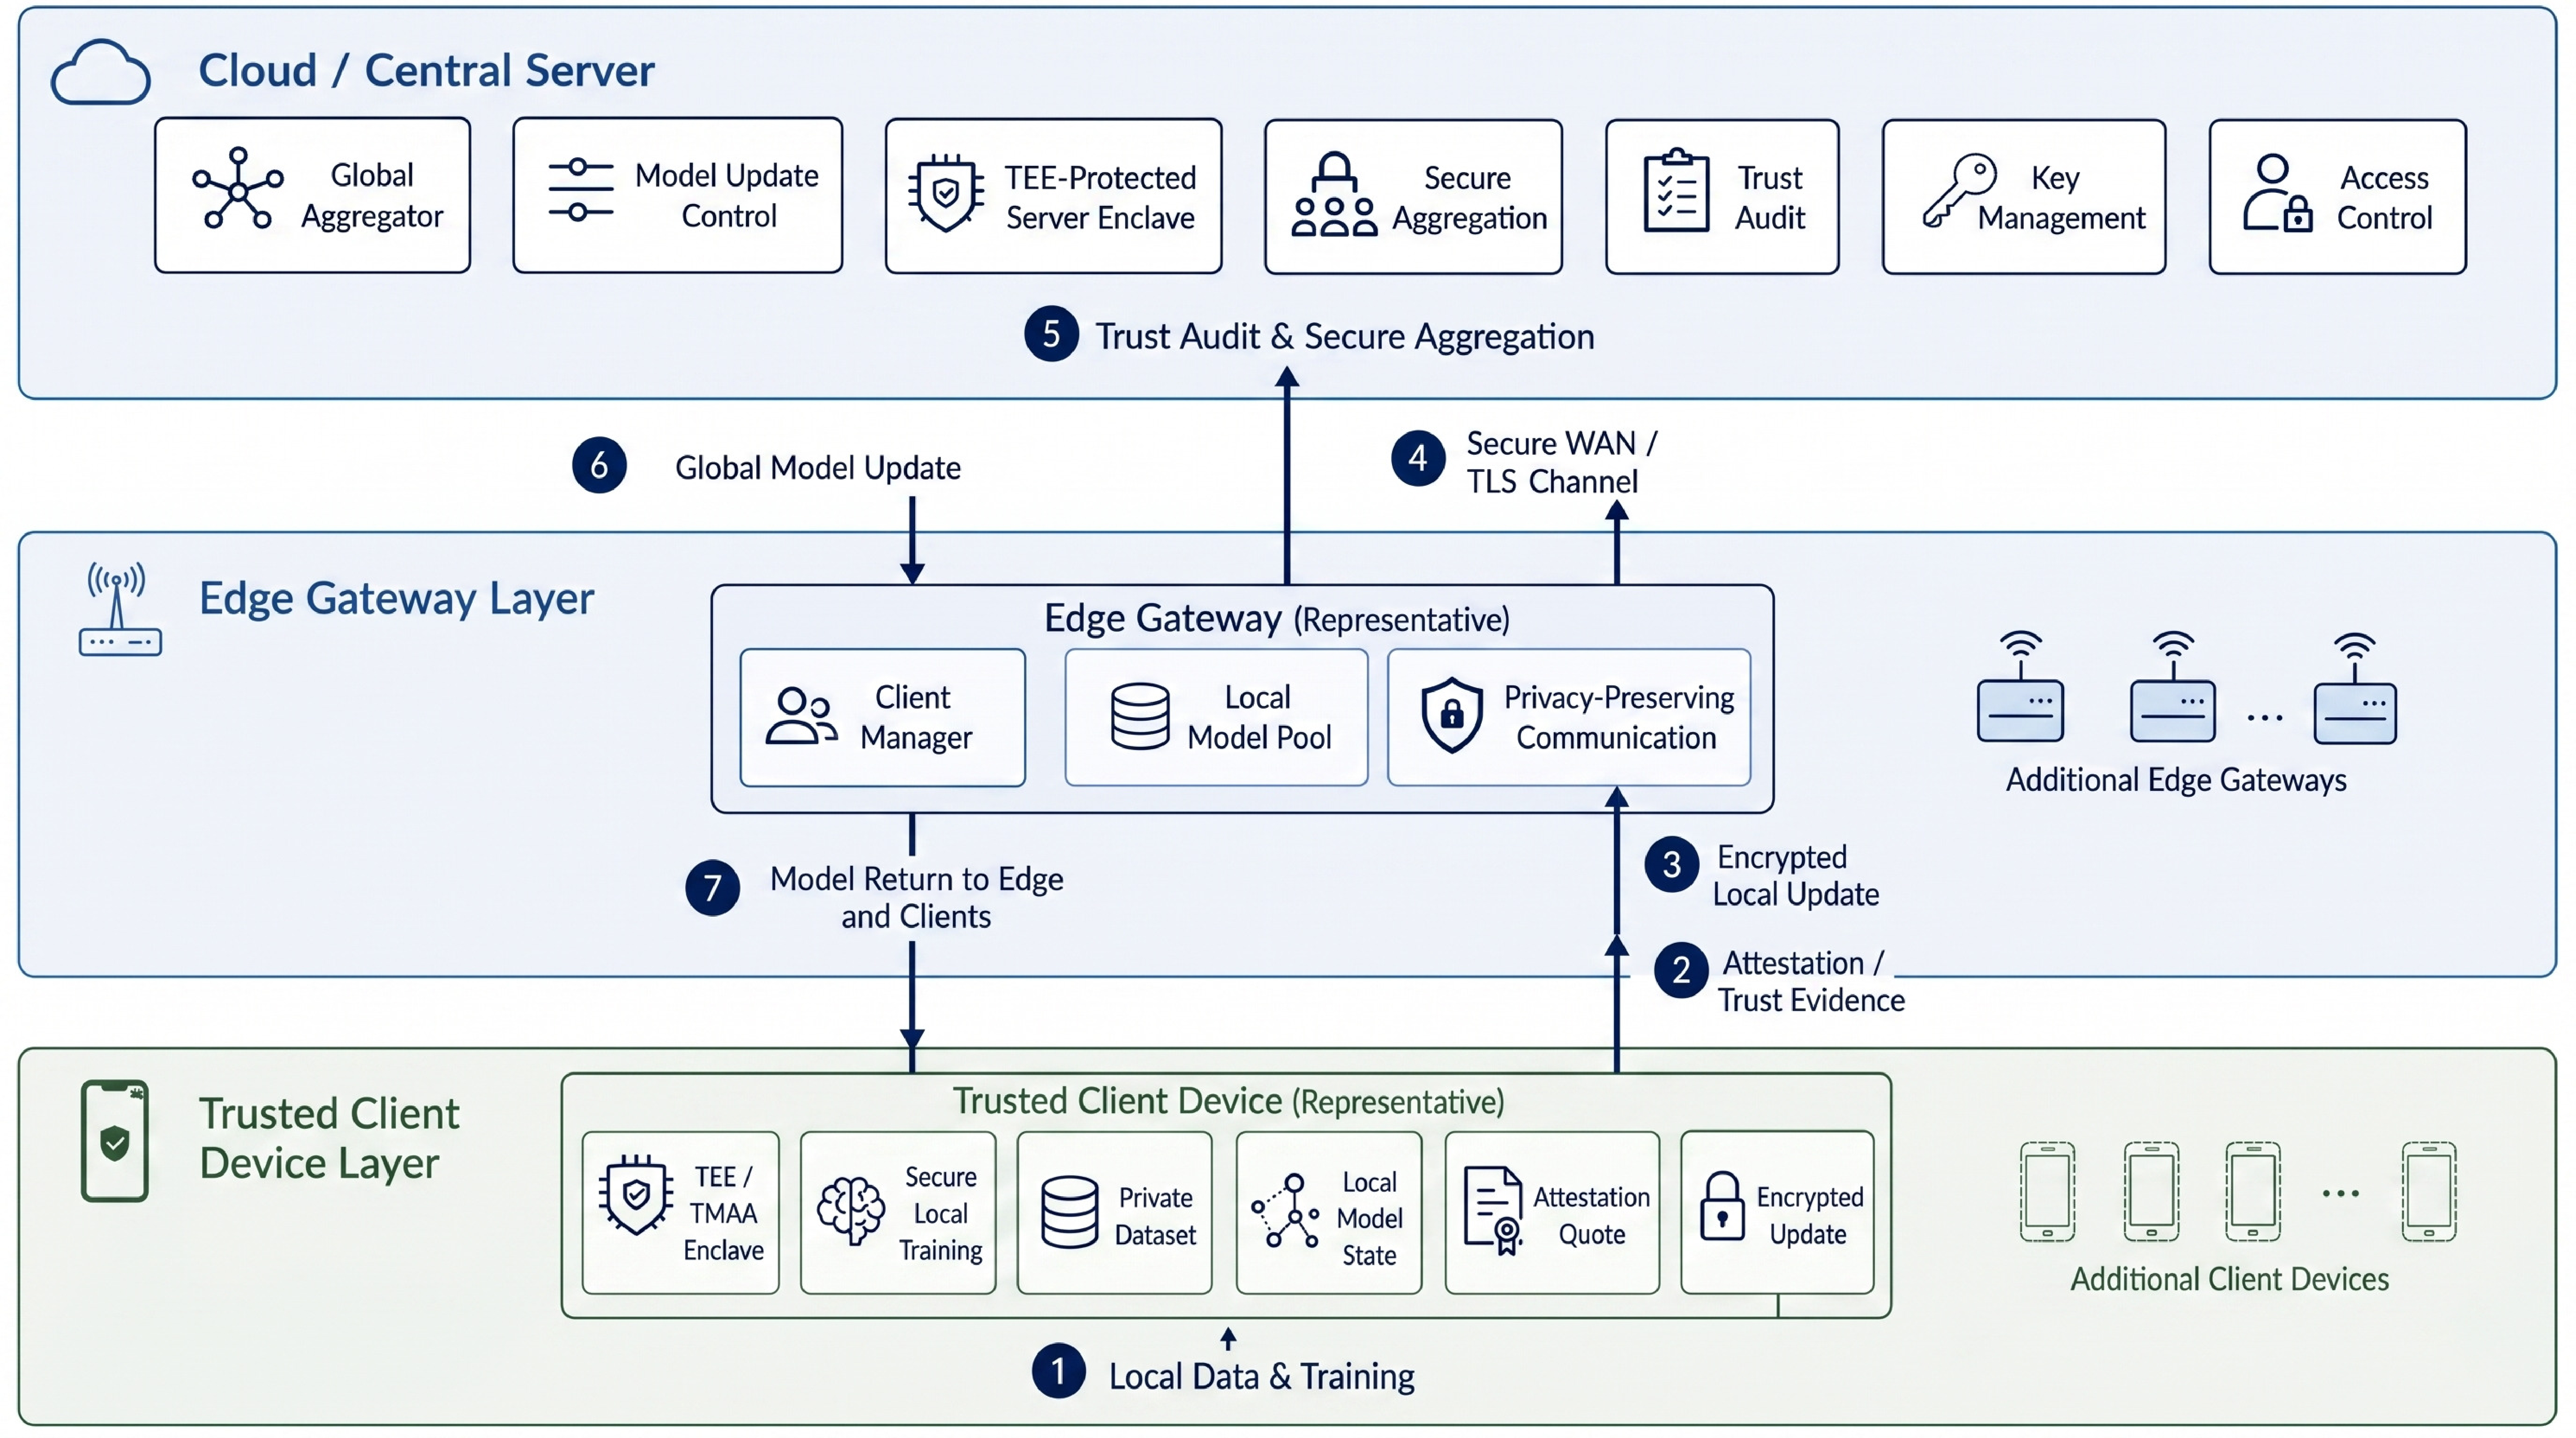
\includegraphics[width=0.90\textwidth]{fig1_system_arch.pdf}
    \caption{Federated computing network interaction: client-edge-cloud collaborative physical architecture based on TEE-anchored encryption}
    \label{fig:system_arch}
\end{figure*}

Based on the network interaction topology above, the proposed trust-flow-driven trusted federated framework builds a complete trust transmission and evaluation chain between the edge and the cloud. The overall workflow of the system and the relationships among its main physical entity modules are defined as follows:

\begin{enumerate}
    \item \textbf{Edge client side (trusted execution and feature extraction)}: Each admitted client must be equipped with a trusted execution environment (TEE) and a trusted management agent (TMAA) deployed inside it. During local training, the TMAA generates an Attestation Quote before training to statically verify the integrity of the execution environment. It also continuously monitors key behavioral feature sequences during training, such as changes in gradient direction and loss fluctuation. Information entropy and Kalman filtering are then used for an initial dynamic trust assessment, which is uploaded to the cloud together with the model update parameters.

    \item \textbf{Central server side (auditing, evolution, and aggregation control)}: As the global coordinator, the server receives client updates and trust evidence, then performs a three-stage coordinated defense based on trust flow. It first conducts \textbf{content auditing}, extracting a clean reference direction and using cosine similarity to calculate high-dimensional update quality. It then enters \textbf{dual-stream state evolution}, where Beta Bayesian inference is used to build a historical utility stream for long-term contribution evaluation, while multidimensional max-value probes update an instant risk stream to identify sudden anomalies. Finally, \textbf{layered robust aggregation} applies differentiated gated clipping and survivor weight re-normalization according to the security sensitivity of different network layers, producing and distributing a globally secure update.
\end{enumerate}

Through the coordinated interaction of the edge and cloud entity modules, the system forms a full-lifecycle physical and logical closed loop: hardware admission control $\to$ runtime feature monitoring $\to$ trust state evolution $\to$ risk-gated aggregation.


\subsection{Composite Threat Assumptions and Strong Trust-Base Boundary (Threat Model)}
To clearly define the boundary between attacker and defender capabilities, this paper adopts the following threat model (see Figure~\ref{fig:threat_model}):
\begin{itemize}
    \item \textbf{Explicit TEE boundary}: Intel and AMD TEE-capable platforms protect attestation-critical code, device keys, report integrity, report freshness, and the trusted monitoring path against a compromised host OS. They do not certify labels, samples, optimization objectives, or semantic intent. Thus, a client can produce a signed poisoned update inside an otherwise valid measured training workflow; post-attestation modification outside that workflow is excluded.
    \item \textbf{Honest-but-curious server}: The server follows the dual-stream and layered-aggregation protocol and may inspect individual updates and audit statistics, but it cannot change the stated transition rules.
    \item \textbf{Internal malicious clients}: An admitted client may perform label flipping, trigger backdoors, clean-label poisoning, semantic poisoning, sign flipping, or gradient scaling. The analytical assumption is fewer than $50\%$ malicious admitted clients; the 50\% experiment is an out-of-assumption stress test, not a Byzantine threshold or a theoretical guarantee. Physical probing and advanced microarchitectural side channels are excluded.
\end{itemize}

\begin{figure*}[t]
    \centering
    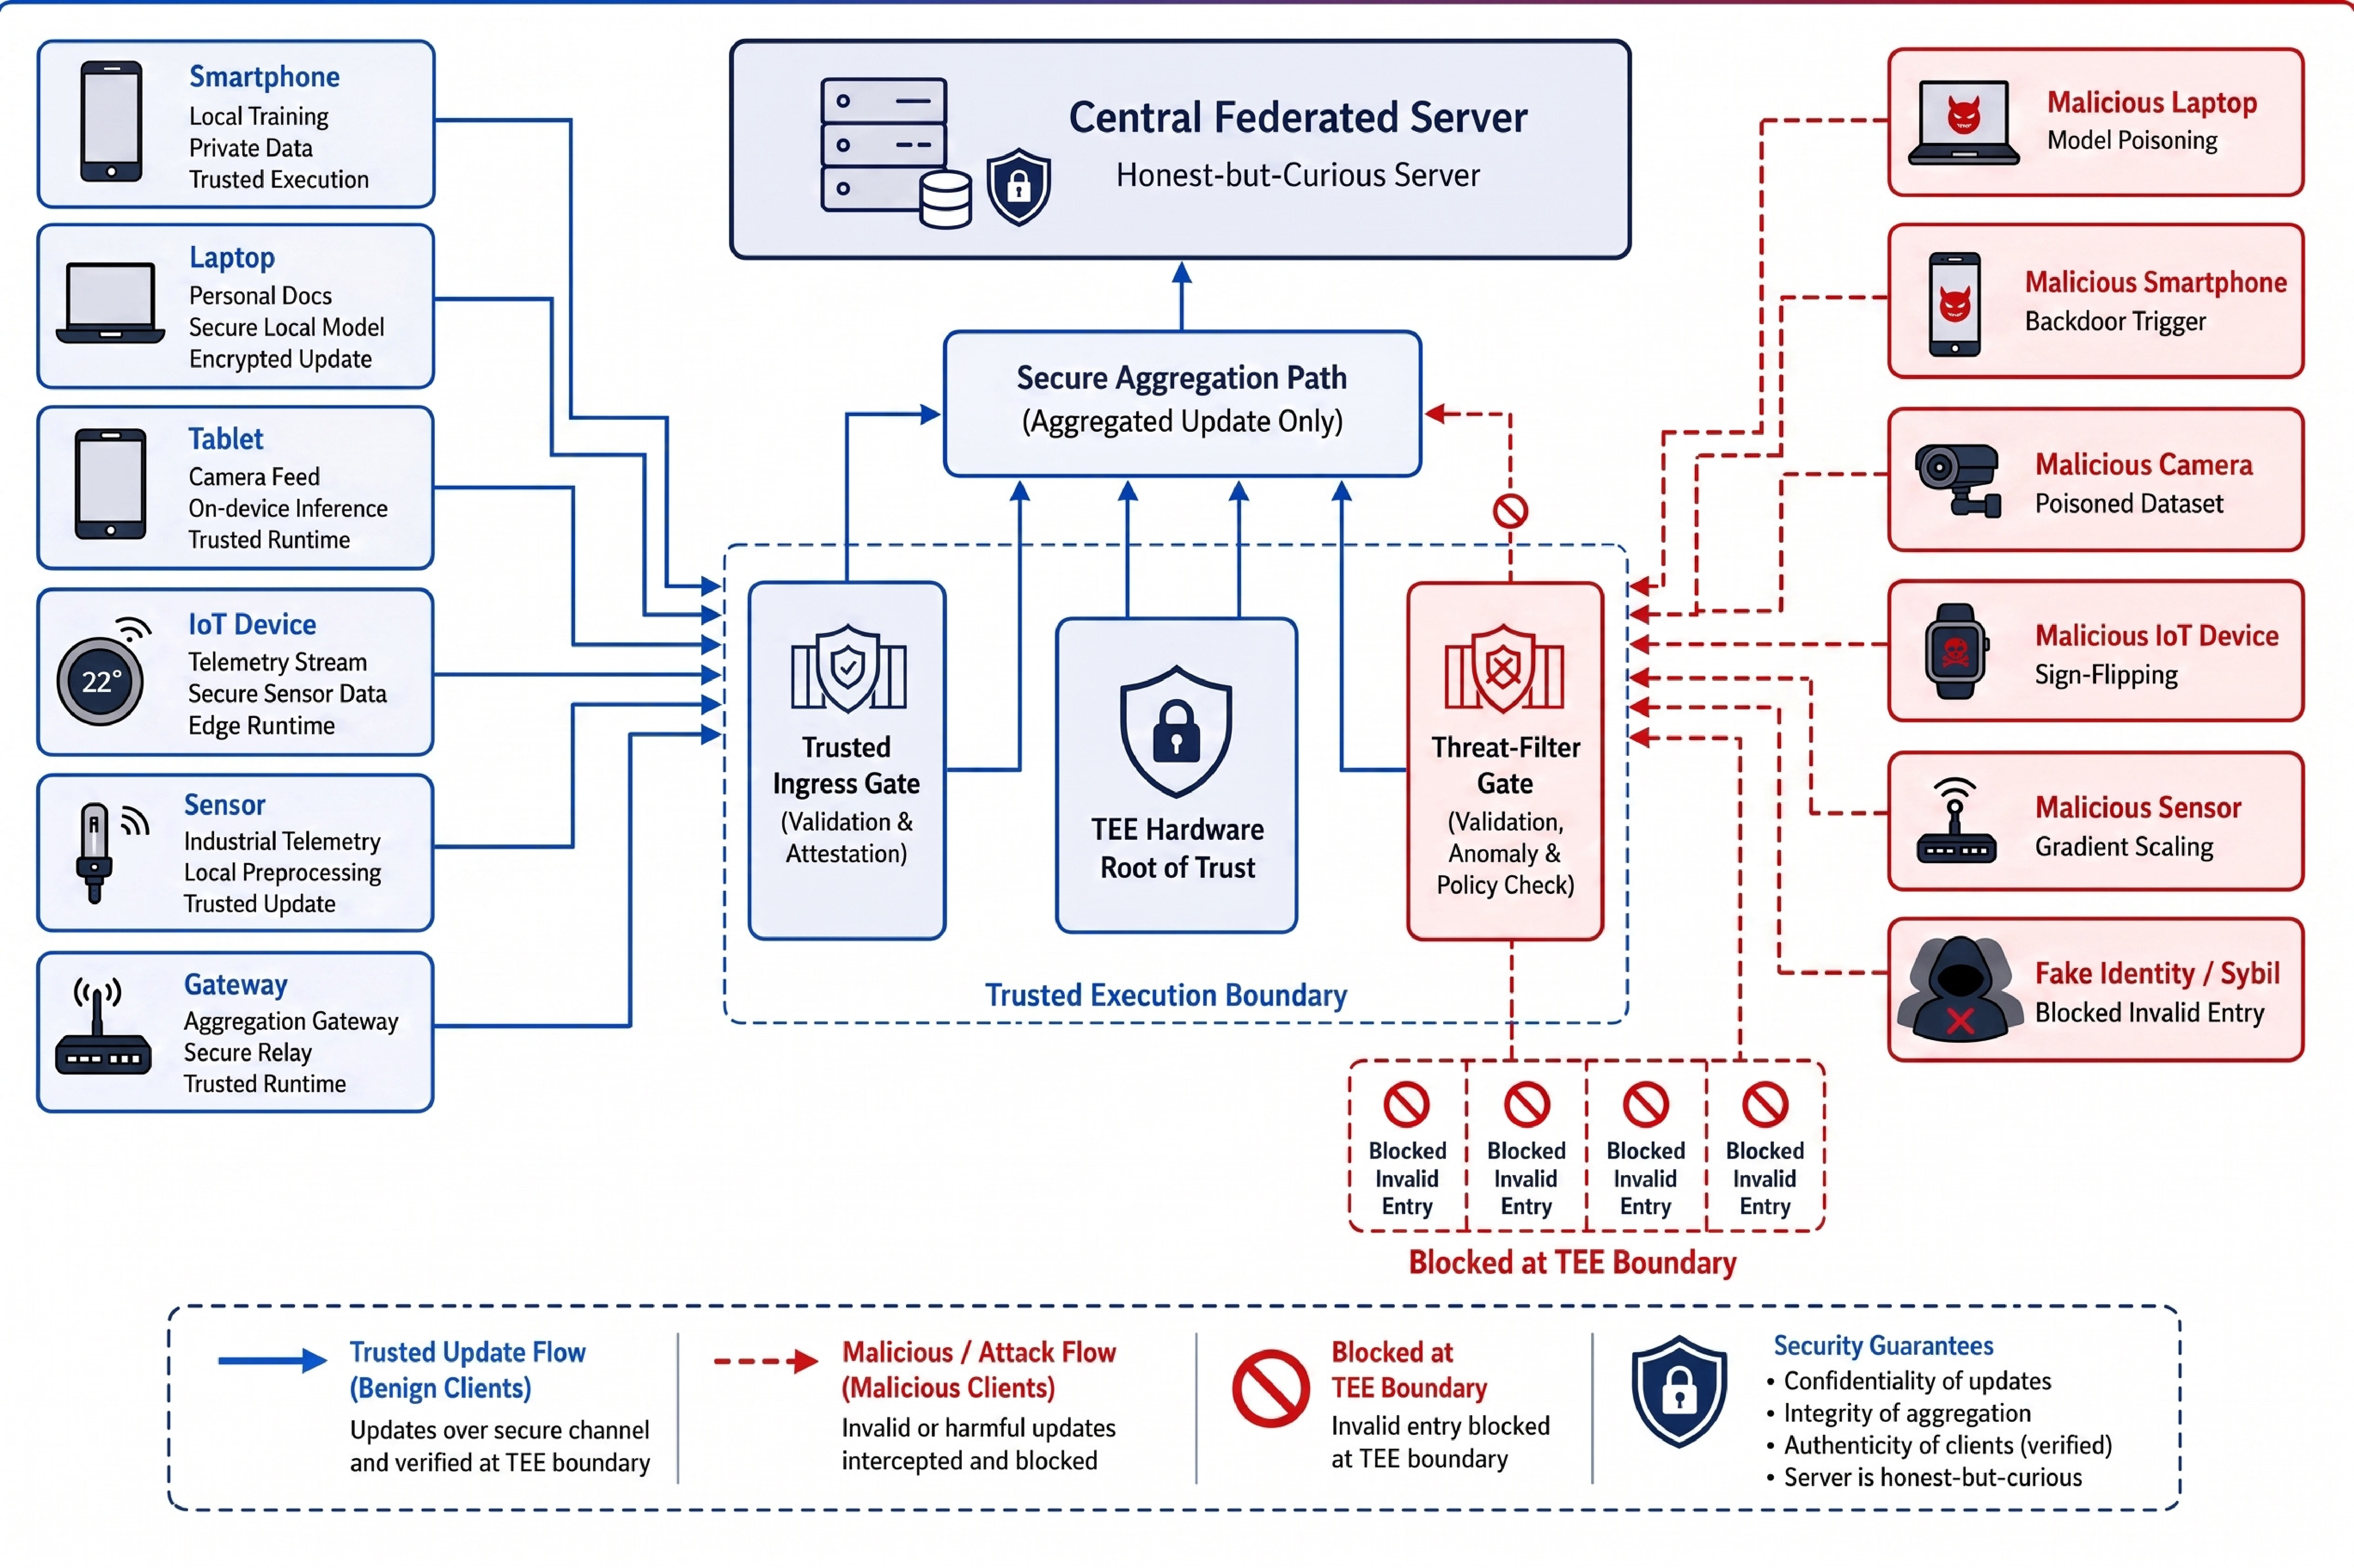
\includegraphics[width=0.88\textwidth]{fig2_threat_model.pdf}
    \caption{Security penetration and multidimensional composite poisoning threat model in an edge wide-area network}
    \label{fig:threat_model}
\end{figure*}

\subsection{Design Goals and System Boundary}
The design goals of the proposed framework are to maintain convergence under
the stated attacks, reduce irreversible false bans of long-tail clients, and
measure server-side trust-flow cost separately from attestation and
cryptographic privacy costs. The term secure aggregation is not used here:
the server must inspect per-client evidence, so cryptographic
privacy-preserving aggregation is outside the system boundary.


\section{Proposed Method: Trust-Flow Framework}

For the threat model above, this paper proposes a trust-flow-driven trusted federated learning framework (see Figure~\ref{fig:framework}). Following the execution order of federated learning, the framework first performs trusted admission and runtime monitoring on the client side, then conducts current-round content auditing and cross-round reputation evolution on the server side, and finally enters layered security control during aggregation. Each training round is therefore divided into four decision stages: admission and runtime monitoring, content auditing, state evolution, and layered aggregation; global model distribution follows as the protocol output. At a higher level of abstraction, these stages correspond to three layers: client admission and monitoring, server auditing and evolution, and aggregation security assurance.

The key of this macro-to-micro structure is the continuous transfer of trust states. Phase one outputs $TrustScore$, indicating whether the client has a trustworthy basis for admission and execution. Phase two outputs $ContentScore$, judging whether the update submitted in the current round deviates from the clean reference and the collaborative direction of the group. Phase three deposits current-round signals into $HistPerf$ and $RiskEMA$, distinguishing long-term low contribution from short-term high risk. Phase four fuses the three types of signals into $RawScore$ and performs differentiated aggregation by network layer. Unlike single-point defenses, data generated at each phase continues to constrain later phases, continuously updating the \textbf{Trust Flow} and forming closed-loop control.

\begin{figure*}[t]
    \centering
    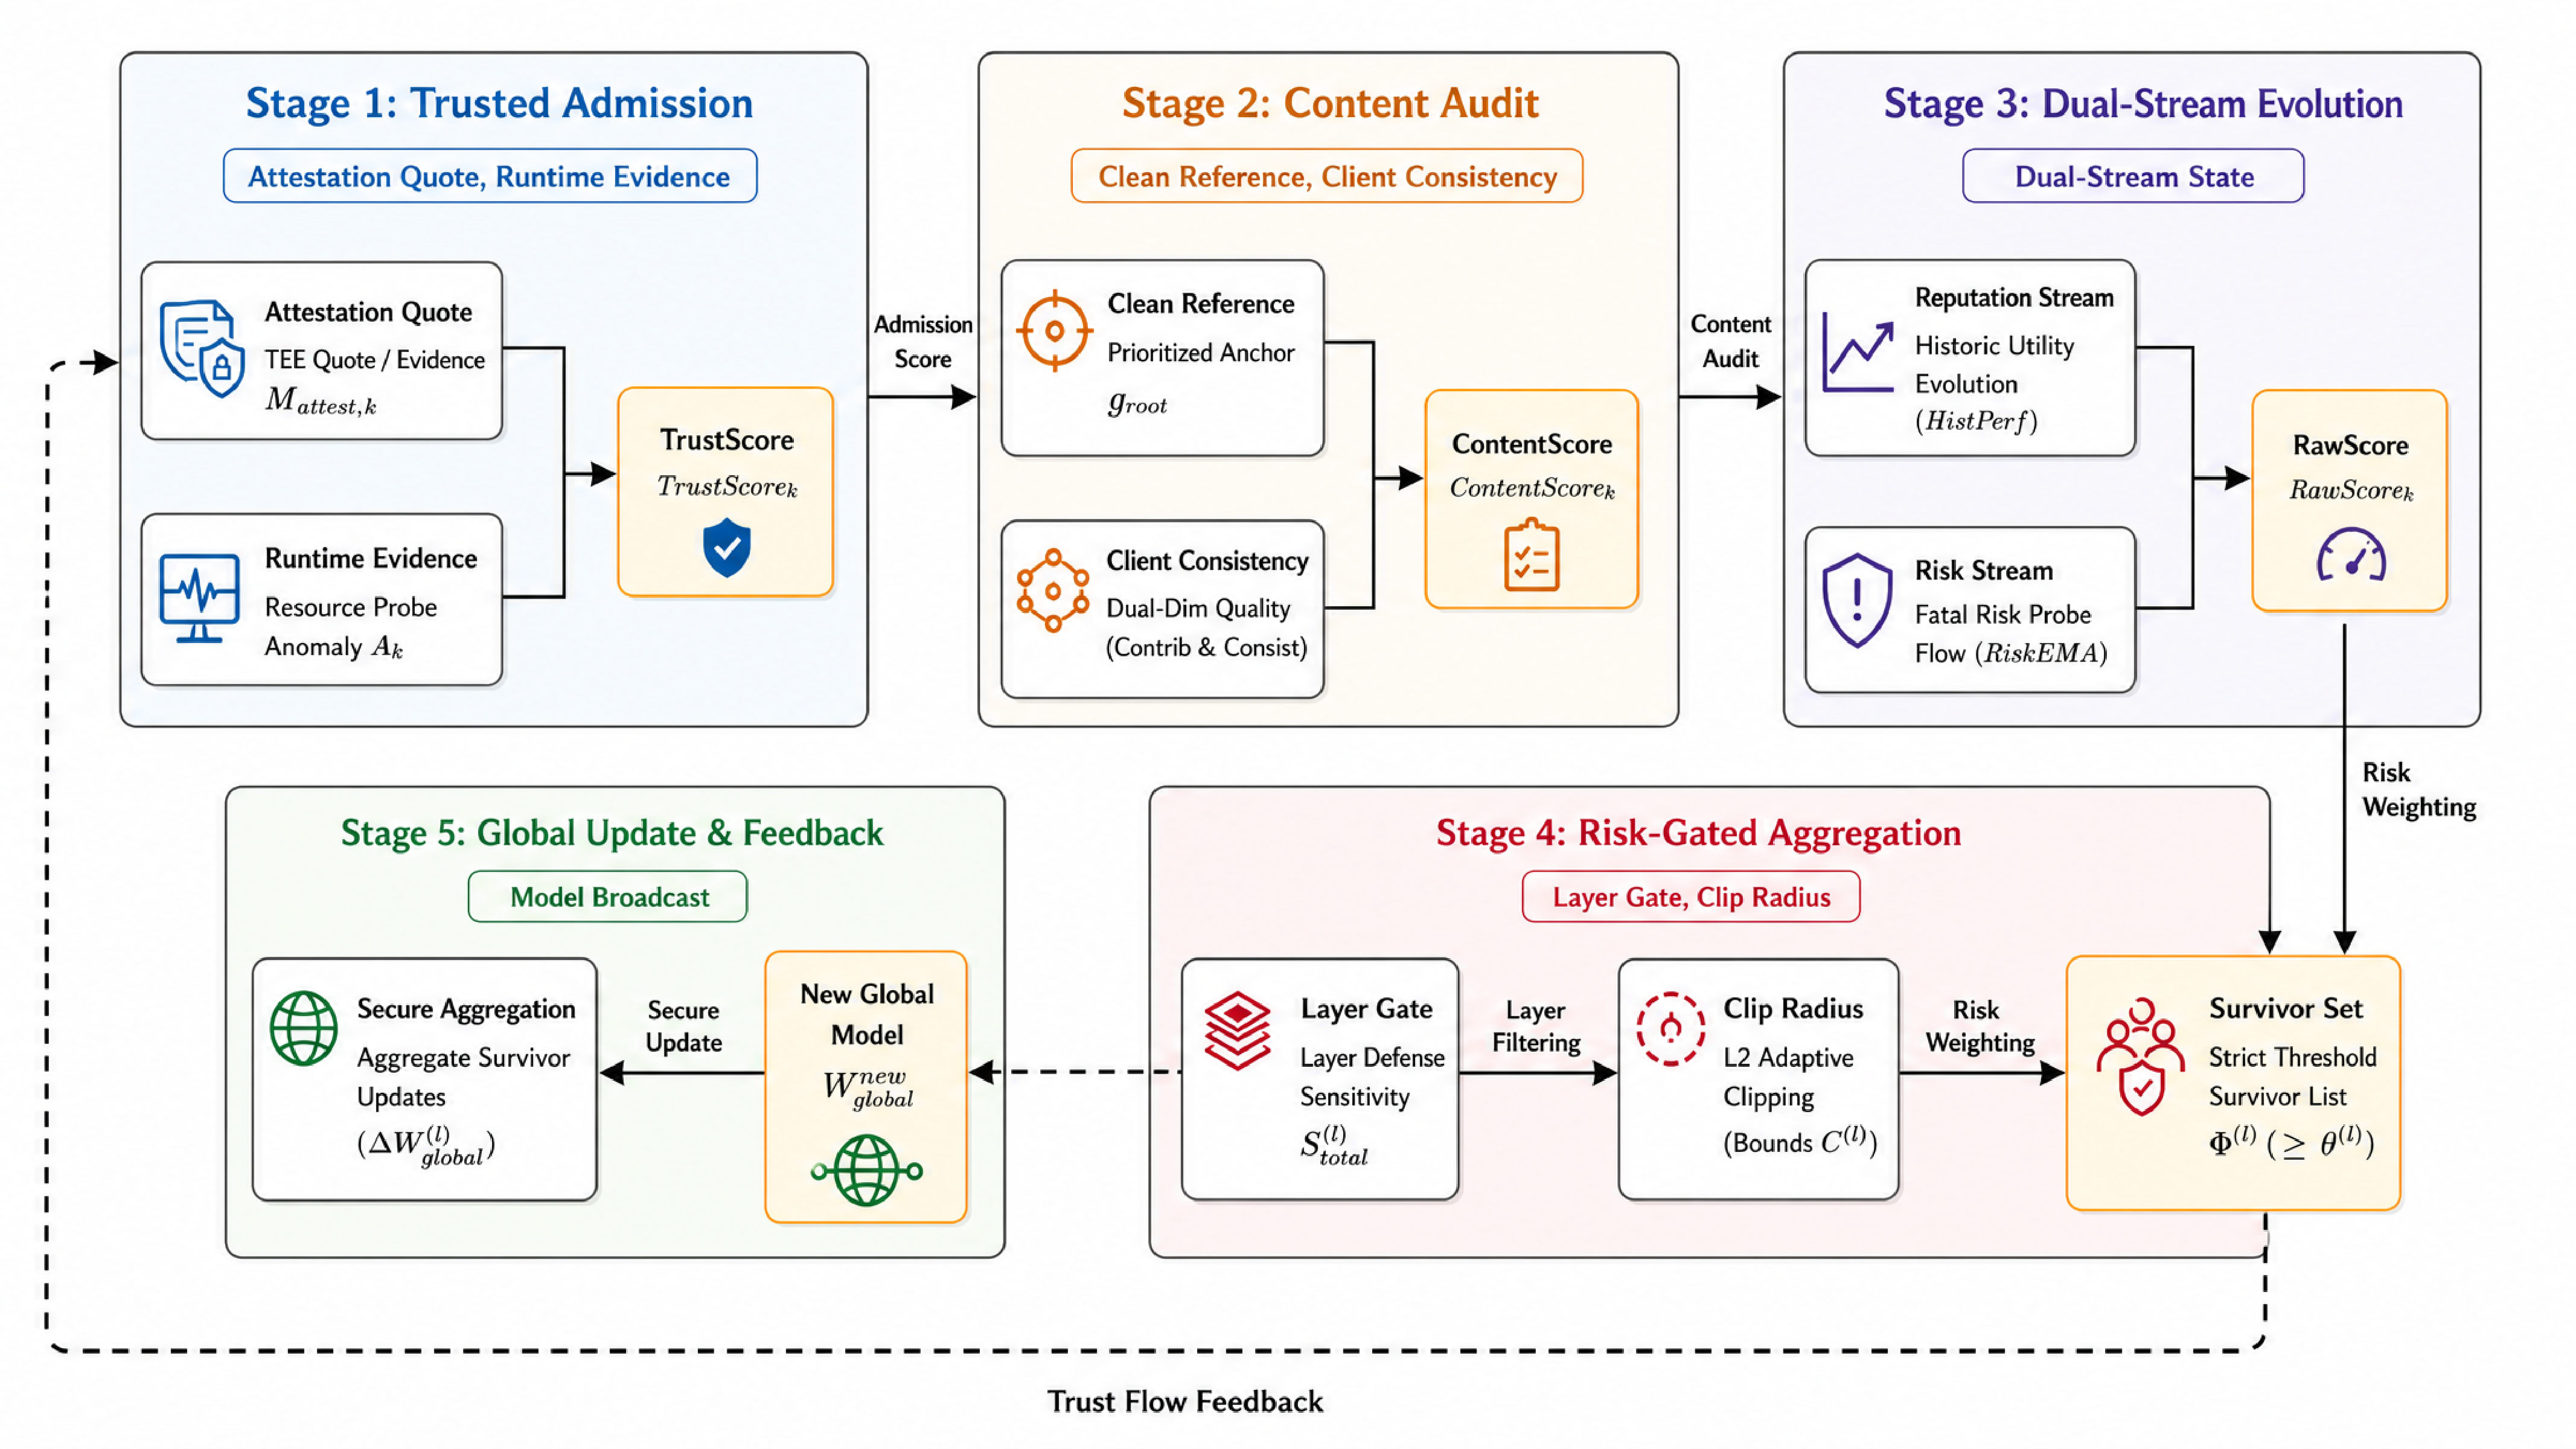
\includegraphics[width=\textwidth]{fig3_arch.pdf}
    \caption{Overview of the four-stage defense loop in trust-flow-driven trusted federated learning}
    \label{fig:framework}
\end{figure*}

To facilitate the following derivation, Table~\ref{tab:notations} lists the definitions of core symbols.

\begin{table*}[t]
    \centering
    \caption{Core system parameters and trust-flow notation}
    \label{tab:notations}
    \renewcommand{\arraystretch}{1.25}
    \setlength{\tabcolsep}{3pt}
    \begin{tabular*}{\textwidth}{@{\extracolsep{\fill}} >{\raggedright\arraybackslash}p{2.8cm} >{\raggedright\arraybackslash}p{4.5cm} >{\raggedright\arraybackslash}p{2.2cm} >{\raggedright\arraybackslash}p{4.5cm}}
        \toprule
        \textbf{Symbol} & \textbf{Definition} & \textbf{Symbol} & \textbf{Definition} \\
        \midrule
        $W_{global}^{(t)}$ & Global model weights in round $t$ & $\mathcal{A}$ & Active node set eligible for valid aggregation in the current round \\
        $\Delta W_k$ & Model gradient/parameter update submitted by client $k$ & $\Phi^{(l)}$ & Valid secure survivor subset at layer $l$ \\
        $TrustScore_k$ & TEE hardware-anchored admission trust score & $HistPerf_k$ & Accumulated state of the historical utility stream ($HistPerf \in [0, 1]$)\\
        $ContentScore_k$ & Current-round content quality score under dual references & $RiskEMA_k$ & Decayed state of the instant risk stream ($RiskEMA \in [0, 1]$)\\
        $RawScore_k$ & Final privilege score after fusing three-dimensional scores and applying risk discounting & $M_{attest,k}$ & Hardware remote attestation verification flag \\
        $g_{root}$ & Clean guiding anchor direction extracted by the server & $A_k$ & Runtime anomaly score of client $k$ in physical resource usage \\
        \bottomrule
    \end{tabular*}
    \renewcommand{\arraystretch}{1.0}
\end{table*}

\subsection{Hardware Admission and Dynamic Trust Assessment}
Admission is a two-stage process: static execution admission and dynamic
evidence tracking. Let $M_{\mathrm{attest},k}\in\{0,1\}$ indicate whether the
attestation report, freshness nonce, and binding to the current round and update
digest are valid. During initialization, the client invokes a device-unique key
and produces a quote containing a vendor-specific measurement digest, code
identity, runtime configuration, round nonce, update digest, and a monotonic
freshness counter. A client that fails this check is rejected before its update
enters statistical aggregation.

During local training, the trusted management and attestation agent monitors
the standardized sequence
$\mathcal{X}_k^{(t)}=\{\Delta\mathrm{grad},\Delta\mathrm{loss},
\mathrm{instr\_dist}\}$. After concatenating the standardized feature
histograms, let $h_k^{(t)}=H(\mathcal{X}_k^{(t)})/H_{\max}\in[0,1]$. We define
the entropy-derived observation variance and observation as
\begin{equation}
    R_k^{(t)}=\exp(\lambda h_k^{(t)}),\qquad
    Z_k^{(t)}=\operatorname{clip}\!\left(
    w_aM_{\mathrm{attest},k}+(1-w_a)(1-h_k^{(t)}),0,1\right),
\end{equation}
where $w_a=0.7$ and $\lambda=1.0$. High entropy represents uncertain evidence;
it is not used as a direct maliciousness label.

The scalar Kalman recursion is
\begin{equation}
    T_k^{-,(t)}=T_k^{(t-1)},\qquad P_k^{-,(t)}=P_k^{(t-1)}+Q,
\end{equation}
\begin{equation}
\begin{aligned}
    K_k^{(t)}&=\frac{P_k^{-,(t)}}{P_k^{-,(t)}+R_k^{(t)}},\\
    T_k^{(t)}&=T_k^{-,(t)}+K_k^{(t)}
        \left(Z_k^{(t)}-T_k^{-,(t)}\right),\\
    P_k^{(t)}&=(1-K_k^{(t)})P_k^{-,(t)}.
\end{aligned}
\end{equation}
Here $Q=0.01$ is the fixed process-noise variance. A fresh admitted client is
initialized with $T_k^{(0)}=1$, $P_k^{(0)}=0.25$, and
$RiskEMA_k^{(0)}=0$. The admission privilege is
\begin{equation}
    TrustScore_k^{(t)}=M_{\mathrm{attest},k}
    \operatorname{clip}\!\left(\frac{T_k^{(t)}}{1+P_k^{(t)}},0,1\right).
\end{equation}
High entropy therefore lowers the Kalman gain and prevents an uncertain
observation from abruptly rewriting cross-round trust. A new client starts in
NORMAL after valid attestation; its first-round evidence is provisional and
cannot trigger an irreversible blacklist.

\subsection{Reference Direction Construction and Consistency Auditing}
Relying only on cosine similarity among clients can be misled by collusion attacks. The server therefore prioritizes a declared clean reference when available. In the reported experiments, a balanced 500-sample proxy set (50 images per CIFAR-10 class) is held by the server, is not included in client training, and is provided to every reference-dependent baseline under the same protocol. The same set supports the guiding gradient, clean-loss probe, and activation probe. If this direction is unavailable, a fallback reference is constructed from high-trust, low-risk admitted clients. The corresponding weight is defined as:
\begin{equation}
    \omega_{k}^{ref} = TrustScore_{k} \cdot (1 - RiskEMA_{k}^{prev})^{2}.
\end{equation}
The final reference direction $g_{root}$ is:
\begin{equation}
    g_{root}=
    \begin{cases}
        g_{root\_clean},                                                      & \text{if server validation direction available}, \\
        \sum_{k} \frac{\omega_{k}^{ref}}{\sum_j \omega_{j}^{ref}} \Delta W_k, & \text{otherwise}.
    \end{cases}
\end{equation}

After obtaining $g_{root}$, the server calculates a content quality score for each client update $\Delta W_k$. This score considers both global contribution, namely consistency with the reference direction, and group consistency, namely the degree of agreement with other high-reputation clients:
\begin{align}
    S_{contrib,k}    & = \max\left(0,\ \alpha_{1} + \alpha_{2} \cdot \cos(\Delta W_{k}, g_{root})\right),                                                              \\
    S_{consist,k}    & = \frac{\sum_{j\neq k} TrustScore_{j} \cdot \xi_{j,k}}{\sum_{j\neq k} TrustScore_{j} + \varepsilon},                                            \\
    ContentScore_{k} & = \frac{(1 + \beta_{fusion}^{2}) \cdot S_{consist,k} \cdot S_{contrib,k}}{\beta_{fusion}^{2}\cdot S_{consist,k} + S_{contrib,k} + \varepsilon}.
\end{align}
Here, $\xi_{j,k}=\max(0,\alpha_1+\alpha_2\cos(\Delta W_k,\Delta W_j))$, and $\alpha_1+\alpha_2=1.0$ adjusts the cosine mapping interval. The parameter $\beta_{fusion}>1.0$, with default $\beta_{fusion}=2.0$, moderately increases the weight assigned to consistency with the clean direction, strengthening resistance to collusive drift. $ContentScore_k$ describes only the content quality of the current-round update and is not equivalent to permanent reputation. For legitimate long-tail nodes under strong Non-IID settings, a low single-round score may result from data skew rather than attack behavior. This score is therefore passed to the cross-round state evolution in phase three, where subsequent handling is jointly determined by the historical utility stream and the instant risk stream.

\begin{algorithm}[htbp]
    \caption{Admission and content auditing based on TEE hardware anchors and clean reference}
    \label{alg:phase12}
    \begin{algorithmic}[1]
        \REQUIRE $\mathcal{C}$, $\{\Delta W_k\}_{k\in\mathcal{C}}$, $RiskEMA^{(t-1)}$
        \ENSURE $TrustScore_k$, $ContentScore_k$, valid reference baseline $g_{root}$
        \STATE \textbf{Phase 1: Hardware Anchoring and Dynamic Trust Measurement}
        \FOR{each client $k \in \mathcal{C}$}
        \IF{$M_{attest,k} == 0$ (TEE remote attestation fails)}
        \STATE Reject admission: $TrustScore_k \leftarrow 0$, and skip this round
        \ELSE
        \STATE \textit{Inside TEE}: record behavior sequence $\mathcal{X}_k = \{ \Delta \text{grad}, \Delta \text{loss}, \text{instr\_dist} \}$
        \STATE Compute information entropy $H_k \leftarrow -\sum p(x_i) \log p(x_i)$
        \STATE Map entropy to measurement noise $R_k \leftarrow \exp(\lambda \cdot H_k)$
        \STATE \textit{Kalman filter update}:
        \STATE Trust estimate $\hat{T}_k$, covariance $P_k \leftarrow \mathrm{KalmanFilter}(H_k, \text{previous state})$
        \STATE Admission trust score $TrustScore_k \leftarrow \hat{T}_k \cdot \frac{1}{1 + P_k}$
        \ENDIF
        \ENDFOR
        \STATE \textbf{Phase 2: Reference Direction Construction and Collaborative Consistency Auditing}
        \IF{server clean validation data are available}
        \STATE Extract true guiding gradient $g_{root} \leftarrow g_{root\_clean}$
        \ELSE
        \STATE Compute nonlinear weight $\omega_k^{ref} \leftarrow TrustScore_k \cdot (1 - RiskEMA_k^{(t-1)})^2$
        \STATE Generate fallback clean anchor $g_{root} \leftarrow \sum_k (\omega_k^{ref} \Delta W_k) / \sum_j \omega_j^{ref}$
        \ENDIF
        \FOR{each admitted active client $k$}
        \STATE Global contribution score $S_{contrib,k} \leftarrow \max(0, \alpha_1 + \alpha_2 \cos(\Delta W_k, g_{root}))$
        \STATE Group collaboration score $S_{consist,k} \leftarrow \frac{\sum_{j \neq k} TrustScore_j \max(0, \alpha_1 + \alpha_2 \cos(\Delta W_k, \Delta W_j))}{\sum_{j \neq k} TrustScore_j + \varepsilon}$
        \STATE Harmonic content score $ContentScore_k \leftarrow \frac{(1+\beta_{fusion}^2)S_{consist,k} S_{contrib,k}}{\beta_{fusion}^2 S_{consist,k} + S_{contrib,k} + \varepsilon}$
        \ENDFOR
        \RETURN $\{TrustScore_k, ContentScore_k, g_{root}\}$
    \end{algorithmic}
\end{algorithm}

\subsection{Dual-Stream Evolution of Historical Utility and Instant Risk}
A single reputation score confuses low utility caused by data skew with high
risk caused by an attack. Trust Flow therefore maintains a slow historical
utility stream and a fast current-risk stream. Let
$q_k^{(t)}=\operatorname{clip}(ContentScore_k^{(t)},0,1)$. The historical stream
uses the decayed Beta update
\begin{equation}
    a_k^{(t)}=\beta_h a_k^{(t-1)}+q_k^{(t)},\quad
    b_k^{(t)}=\beta_h b_k^{(t-1)}+1-q_k^{(t)},\quad
    HistPerf_k^{(t)}=\frac{a_k^{(t)}}{a_k^{(t)}+b_k^{(t)}+\varepsilon}.
\end{equation}
A fresh client starts with $a_k^{(0)}=b_k^{(0)}=1$, so
$HistPerf_k^{(0)}=0.5$. The decay factor $\beta_h\in(0,1)$ is fixed before the
test rounds. The historical stream reduces privilege gradually and allows a
legitimate long-tail client to recover.

The short-term risk stream is
\begin{equation}
    RiskEMA_k^{(t)}=\beta_rRiskEMA_k^{(t-1)}
    +(1-\beta_r)Risk_k^{inst},
\end{equation}
where $Risk_k^{inst}$ is the maximum current probe. A fresh, validly attested
client starts in NORMAL. Let
$u_k^{(t)}=1-HistPerf_k^{(t)}$ and
$r_k^{(t)}=RiskEMA_k^{(t)}$. The thresholds
$(\tau_h,\tau_s,\tau_q,\tau_b)=(0.26,0.64,0.80,0.90)$ govern utility deficit,
soft risk, quarantine, and blacklisting. A NORMAL client enters SUSPECT after
two consecutive rounds with $u_k^{(t)}>\tau_h$ or $r_k^{(t)}\geq\tau_s$. A
SUSPECT client enters QUARANTINE after three such consecutive rounds or one
current probe with $Risk_k^{inst}\geq\tau_q$. A QUARANTINE client enters
BLACKLIST after four consecutive rounds with $r_k^{(t)}\geq\tau_b$. Recovery
from SUSPECT or QUARANTINE requires two consecutive rounds with
$u_k^{(t)}\leq\tau_h$ and $r_k^{(t)}<\tau_s$; BLACKLIST is irreversible within
an experiment. Counters reset when their conditions are not met, and the state
update is completed before layer aggregation. First-round evidence can reduce
the current update privilege but cannot trigger an irreversible blacklist.

The streams meet only in the aggregation privilege:
\begin{align}
    RawScore_k^{(t)} &=(TrustScore_k^{(t)})^\alpha
    (ContentScore_k^{(t)})^\beta(HistPerf_k^{(t)})^\gamma
    (1-RiskEMA_k^{(t)})^p.
\end{align}
This timing allows current risk to veto a sleeper burst despite high history,
while a low-similarity benign client remains recoverable through the slow stream.

\subsection{Risk-Gated Layered Aggregation}
Backdoors may concentrate in deep layers, while shallow feature layers can
carry useful heterogeneous information. Trust Flow therefore assigns each
layer $l$ a sensitivity score. With $L$ total layers, define
\begin{align}
    S_{priv}^{(l)}&=\exp(-\tau_p l/L),\qquad
    S_{util}^{(l)}=\frac{\|g_{root}^{(l)}\|_2}
    {\max_m\|g_{root}^{(m)}\|_2+\varepsilon},\\
    S_{sec}^{(l)}&=\frac{1}{2}\left(1-\frac{1}{|\mathcal{T}|}
    \sum_{k\in\mathcal{T}}\cos(\Delta W_k^{(l)},g_{root}^{(l)})\right).
\end{align}
Here
$\mathcal{T}=\{k\in\mathcal{A}:M_{\mathrm{attest},k}=1,\,
RiskEMA_k^{(t-1)}<\tau_s\}$ is the trusted reference set. If it is empty, the
server uses $\mathcal{A}$ only for normalization and records the absence of a
trusted peer reference. Thus $S_{priv}^{(l)}$, $1-S_{util}^{(l)}$, and
$S_{sec}^{(l)}$ lie in $[0,1]$. We set
\begin{equation}
    S_{total}^{(l)}=w_pS_{priv}^{(l)}+w_u(1-S_{util}^{(l)})
    +w_sS_{sec}^{(l)},\qquad (w_p,w_u,w_s)=(0.3,0.3,0.4).
\end{equation}
The layer threshold and clipping radius are
\begin{equation}
    \theta^{(l)}=\mu_{base}+\lambda_sS_{total}^{(l)},\qquad
    C^{(l)}=\frac{C_{base}}{S_{total}^{(l)}+\varepsilon_c},
\end{equation}
where $\tau_p=3.0$ and $C_{base}$ is the median trusted-client update norm.
A layer with stronger suspicious drift is therefore harder to enter and more
tightly clipped.

Survivors are
$\Phi^{(l)}=\{k\in\mathcal{A}:RawScore_k^{(t)}\geq\theta^{(l)}\}$. To preserve
the stated global objective, data-volume weights are retained:
\begin{equation}
    \tilde{w}_k^{(l)}=
    \frac{p_kRawScore_k^{(t)}}{\sum_{j\in\Phi^{(l)}}p_jRawScore_j^{(t)}
    +\varepsilon},\qquad
    \widehat{\Delta W}_k^{(l)}=
    \frac{\Delta W_k^{(l)}}{\max(1,\|\Delta W_k^{(l)}\|_2/C^{(l)})}.
\end{equation}
The layer update is
$\Delta W_{\mathrm{global}}^{(l)}
=\sum_{k\in\Phi^{(l)}}\tilde{w}_k^{(l)}
\widehat{\Delta W}_k^{(l)}$. If no client survives, the client with maximum
$RawScore$ is retained with unit normalized weight and the same clipping radius.
Re-normalization prevents the removal of risky clients from silently reducing
the effective learning rate.

\subsection{Model Update Distribution and Knowledge Retention}
Upon the completion of layered aggregation, the server applies the screened increment to the global model, $W_{global}^{new}=W_{global}^{old}+\Delta W_{global}$, and distributes the updated model together with the retained client states, including $HistPerf$. This closes the control loop for the stated protocol; convergence and attack suppression remain empirical properties evaluated in the experiments.

\subsection{Interpretation of the Dual-Stream Design}
The historical stream acts as a low-pass filter for benign content variation,
whereas the maximum probe and the risk EMA preserve abrupt warnings. Under
bounded benign fluctuations and persistent attack evidence, this separation
explains why a long-tail client can recover while a sleeper burst is rapidly
down-weighted. These observations are design properties under the stated
thresholds; they are not a theorem guaranteeing zero FPR or universal Byzantine
robustness. Formal guarantees would require distributional assumptions and
attack models beyond the present empirical scope.

\section{Experiments and Analysis}
\label{sec:experiments}
\subsection{Experimental Setup and Reproducible Parameters}

\subsubsection{Baseline Environment and Hardware-Software Stack}
The experiments use Flower 1.5.0 and PyTorch on CIFAR-10 with a
CIFAR-10-adapted ResNet-18. The first convolution uses a $3\times3$ kernel
with stride one, the initial max-pooling layer is removed, and the classifier
has ten outputs. Training and trusted execution use two real hardware
configurations based on Intel and AMD TEE-capable processors. NVIDIA A10 GPUs
execute model training, while CPU-side TEEs isolate attestation, trusted
monitoring, report generation, and admission-state processing. Both platforms
execute the same request/response protocol, nonce-based freshness verification,
measured-code identity checking, round and update-digest binding, protected
report generation, and admission decision. The testbed consists of anonymized
dual-CPU servers and five NVIDIA A10 GPUs, running Ubuntu 20.04.6 LTS and CUDA
12.8.

Five independent seeds are run on each platform. Aggregate means and standard
deviations are computed over the resulting ten platform-seed runs, while
state trajectories use one fixed seed per platform for readability. The
reported runtime measures server-side aggregation and auditing; it excludes
client communication, enclave transitions, memory pressure, and
vendor-specific attestation latency.

\subsubsection{Dataset Heterogeneous Partitioning}
The 50,000 CIFAR-10 training images are partitioned into a shared 5,000-image
client pool, replicated as a common base subset for all clients, and 45,000
exclusive images: clients 0--9 use an IID split, clients 10--14 use a Dirichlet
partition with $\alpha=1.0$, and clients 15--19 use a strong long-tail partition
with $\alpha=0.1$. Separately, the server holds a balanced 500-image proxy
set (50 per class) from CIFAR-10 test data; it is not used in client training and
is provided to every reference-dependent baseline. FedAvg, Krum, and Trimmed
Mean do not consume the proxy set. This separation makes the clean-data
assumption explicit and distinguishes the shared client-training pool from the
server-side audit reference.

\subsubsection{Malicious Attack Instances and Proportions}
The formal 30\% setting injects six malicious clients into 20 admitted clients.
The six behaviors are active concurrently in every local training round. Client
0 performs untargeted label flipping with $\gamma=0.5$. Client 1 injects a
fixed $3\times3$ lower-right trigger into 20\% of local samples and targets
class 0. Client 2 applies label-preserving clean-label perturbations to 20\% of
local samples with the same target. Client 3 applies a fixed semantic attribute
bias to 20\% of local samples and assigns the biased subset to class 0. Client
4 performs untargeted sign flipping, and Client 5 scales its update by a factor
of 100. Clients 1--3 are targeted attacks; Clients 0, 4, and 5 are evaluated
through clean loss, convergence, and state-transition metrics. Five Sybil nodes
without valid certificates and three free-rider nodes with forged low workload
are used only to validate Phase-One gating and are intercepted before
statistical aggregation. Malicious updates that pass attestation represent an
attacker operating inside an admissible training workflow; post-attestation
host tampering is excluded by the threat model. Each run uses 30 rounds and
three local epochs.

For each targeted behavior $a\in\{\mathrm{trigger},\mathrm{clean},\mathrm{semantic}\}$,
let $\mathcal{B}_a$ be its trigger- or attribute-bearing test subset and
$y_a^*$ its target. We define
$ASR_a=|\{x\in\mathcal{B}_a:\arg\max f(x)=y_a^*\}|/|\mathcal{B}_a|$
and report $ASR_{\mathrm{target}}=\frac{1}{3}\sum_a ASR_a$. The three
attack-specific values are retained in the convergence traces. Untargeted
label, sign, and scaling attacks are evaluated separately through clean
accuracy, loss, and state-transition time.

\textbf{Preemptive Interception Clarification}: The aforementioned eight external infiltration or resource fraud nodes are uniformly intercepted during the protocol phase. They either fail the TMAA hardware gating ($M_{attest,k}=0$) or see their $TrustScore_k \to 0$ owing to anomalous behaviors. Consequently, the 20 nodes statistically analyzed in subsequent sections represent the official participants that successfully navigated the Phase One admission.

The global hyperparameters and defensive component configurations employed in the experiment are delineated in Table~\ref{tab:hyperparams}.

\begin{table*}[t]
    \centering
    \caption{Global Hyperparameters and Defense Component Configuration}
    \label{tab:hyperparams}
    {\small
        \setlength{\tabcolsep}{3pt}
        \begin{tabular*}{\textwidth}{@{\extracolsep{\fill}} >{\raggedright\arraybackslash}p{3.1cm} >{\raggedright\arraybackslash}p{7.8cm} >{\raggedright\arraybackslash}p{3.2cm}}
            \toprule
            \textbf{Module}                              & \textbf{Hyperparameter Description}                         & \textbf{Value}  \\
            \midrule
            \multirow{2}{*}{\shortstack[l]{\textbf{Base}\\\textbf{Environment}}}       & Total nodes in heterogeneous topology ($K$)                                  & $20$            \\
            & Local SGD parameters ($lr$, $Momentum$)                      & $0.001$, $0.9$       \\
            \midrule
            \multirow{6}{*}{\shortstack[l]{\textbf{Admission}\\\textbf{and State}}} & Admission weight $w_a$, entropy scale $\lambda$, process noise $Q$ & $0.7$, $1.0$, $0.01$ \\
            & Initialization $(T_0,P_0,RiskEMA_0)$ & $(1,0.25,0)$ \\
            & 2D audit mapping $\alpha_1, \alpha_2$ and $\beta_{fusion}$ & $0.6$, $0.4$, $2.0$  \\
            & History smoothing $\beta_h$ and risk half-life $\beta_r$             & $0.9$, $0.85$        \\
            & State thresholds $(\tau_h,\tau_s,\tau_q,\tau_b)$ & $0.26,0.64,0.80,0.90$ \\
            & Persistence for SUSPECT/QUARANTINE/BLACKLIST & $2,3,4$ rounds \\
            \midrule
            \multirow{3}{*}{\shortstack[l]{\textbf{Layer Gating}\\\textbf{Phase 4}}}         & Score fusion exponents ($\alpha, \beta, \gamma, p$)             & $3.0, 1.0, 0.5, 1.0$ \\
            & Threshold lower bound $\mu_{base}$ and penalty scale $\lambda_s$          & $0.4$, $1.2$         \\
            & Sensitivity weights $(\tau_p,w_p,w_u,w_s)$ & $(3.0,0.3,0.3,0.4)$ \\
            \bottomrule
        \end{tabular*}
    }
\end{table*}

\textbf{Execution Details}: Each run executes 30 rounds of federated training,
with 3 local epochs per round. Aggregate accuracy and ASR use the ten
platform--seed runs; trajectory charts use one fixed seed per platform. No
interpolation smoothing is applied. The reported duration is a server-side
aggregation and audit measurement rather than an end-to-end deployment time.

\subsection{Empirical Analysis of Defense Effectiveness}

\subsubsection{Global Convergence and Attack Prevention Performance}
As illustrated in Figure~\ref{fig:convergence}, under a 30\% malicious proportion, the model accuracy converges steadily to 92.31\%, while the backdoor ASR plummets to 10.21\%.

\begin{figure*}[t]
    \centering
    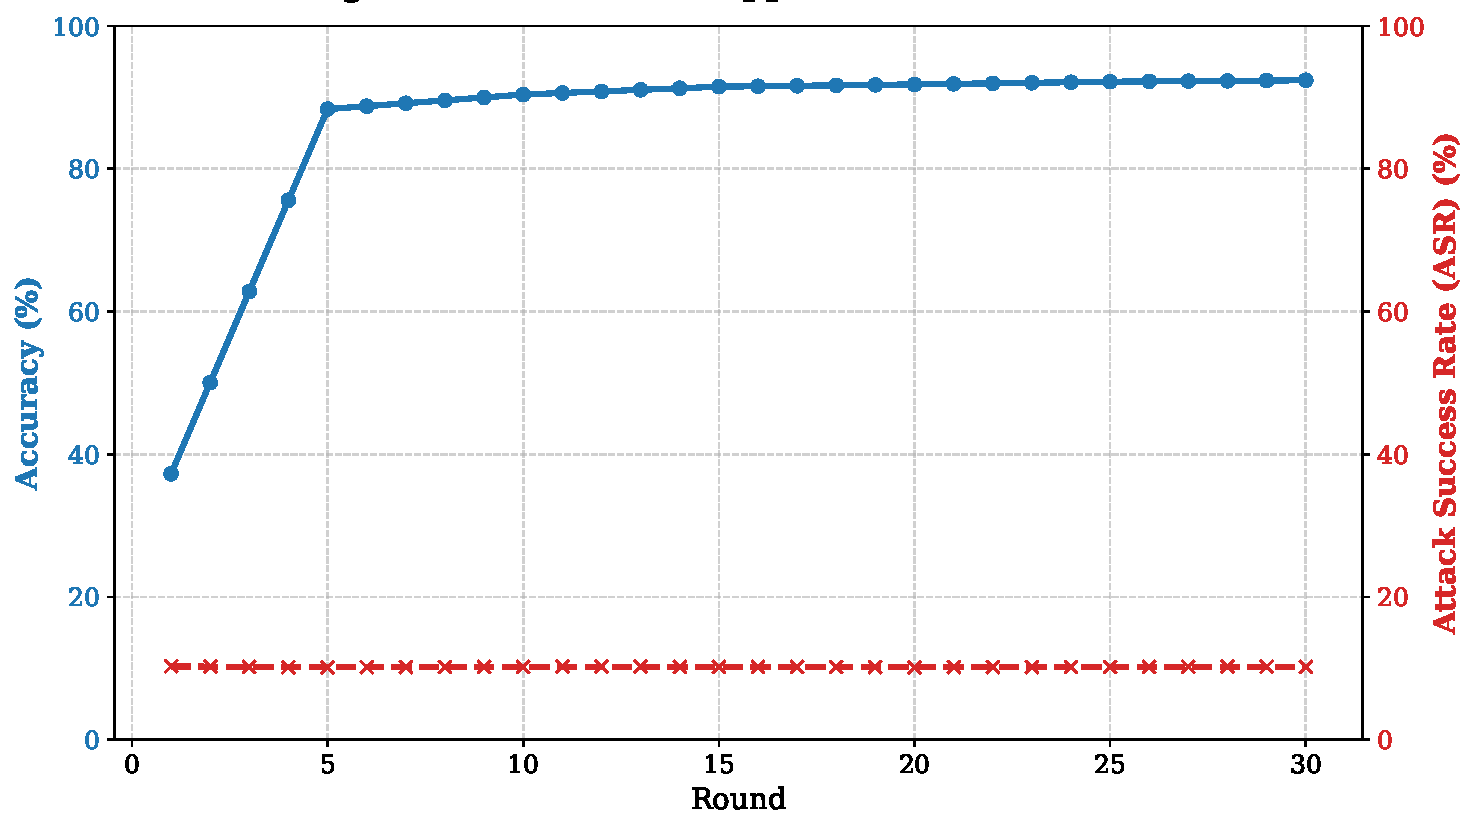
\includegraphics[width=0.85\textwidth]{fig6_convergence_asr.pdf}
    \caption{Global Convergence Accuracy and Backdoor ASR Evolution Curves}
    \label{fig:convergence}
\end{figure*}

\textbf{Statistical Reliability Clarification}: This section and subsequent
aggregate metrics use the mean and standard deviation over ten platform--seed
runs. The node trajectory charts originate from one fixed seed per platform.

\textbf{50\% Malicious Proportion Stress Test}: Because the analytical assumption is fewer than 50\% malicious admitted clients, an auxiliary \textit{Flwr-half} environment with 10 malicious and 10 legitimate nodes is reported only as an out-of-assumption stress test. It is not used to infer a theoretical boundary. The outcomes are detailed in Table~\ref{tab:half_malicious}.

\begin{table*}[t]
    \centering
    \caption{\textbf{Extreme 50\% Malicious Ratio Stress Test vs. Standard 30\% Baseline}}
    \vspace{4pt}
    \label{tab:half_malicious}
    {\small
        \setlength{\tabcolsep}{3pt}
        \begin{tabular*}{\textwidth}{@{\extracolsep{\fill}} >{\raggedright\arraybackslash}p{5.1cm} c c c c}
            \toprule
            \textbf{Setting}                    & \textbf{Acc (\%)}         & \textbf{ASR (\%)}         & \textbf{TPR (\%)} & \textbf{FPR (\%)} \\
            \midrule
            Standard Baseline (30\% malicious, 6/20)           & 92.31 $\pm 0.09$          & 10.21 $\pm 0.05$          & 100               & 0.00              \\
            \textbf{Stress Test (50\% malicious, 10/20)} & \textbf{91.81 $\pm 0.10$} & \textbf{10.46 $\pm 0.06$} & \textbf{100}      & \textbf{0.00}     \\
            \bottomrule
        \end{tabular*}
    }
\end{table*}

In this stress test, the framework reaches 91.81\% accuracy and 10.46\% targeted ASR, while all 10 malicious nodes are removed under the final-ban metric and no legitimate node is permanently banned in the tested run. The 30-round loss trajectory is a descriptive observation of this configuration; it does not constitute a guarantee outside the stated threat model.

\subsubsection{Trust Flow Tracing and Malicious Node Banning Analysis}
Figure~\ref{fig:node_state} shows representative state trajectories for
explicit poisoning, trigger and semantic backdoors, parameter attacks, and one
benign long-tail client. The attack clients accumulate risk through the
direction, amplitude, clean-loss, activation, or peer probes and are eventually
quarantined or blacklisted according to the persistence rules. The long-tail
client may enter SUSPECT or QUARANTINE after a low content score, but it
recovers when the risk stream does not persist. These trajectories illustrate
the state machine under one fixed seed; they are not universal detection-time
claims.

\begin{figure*}[t]
    \centering
    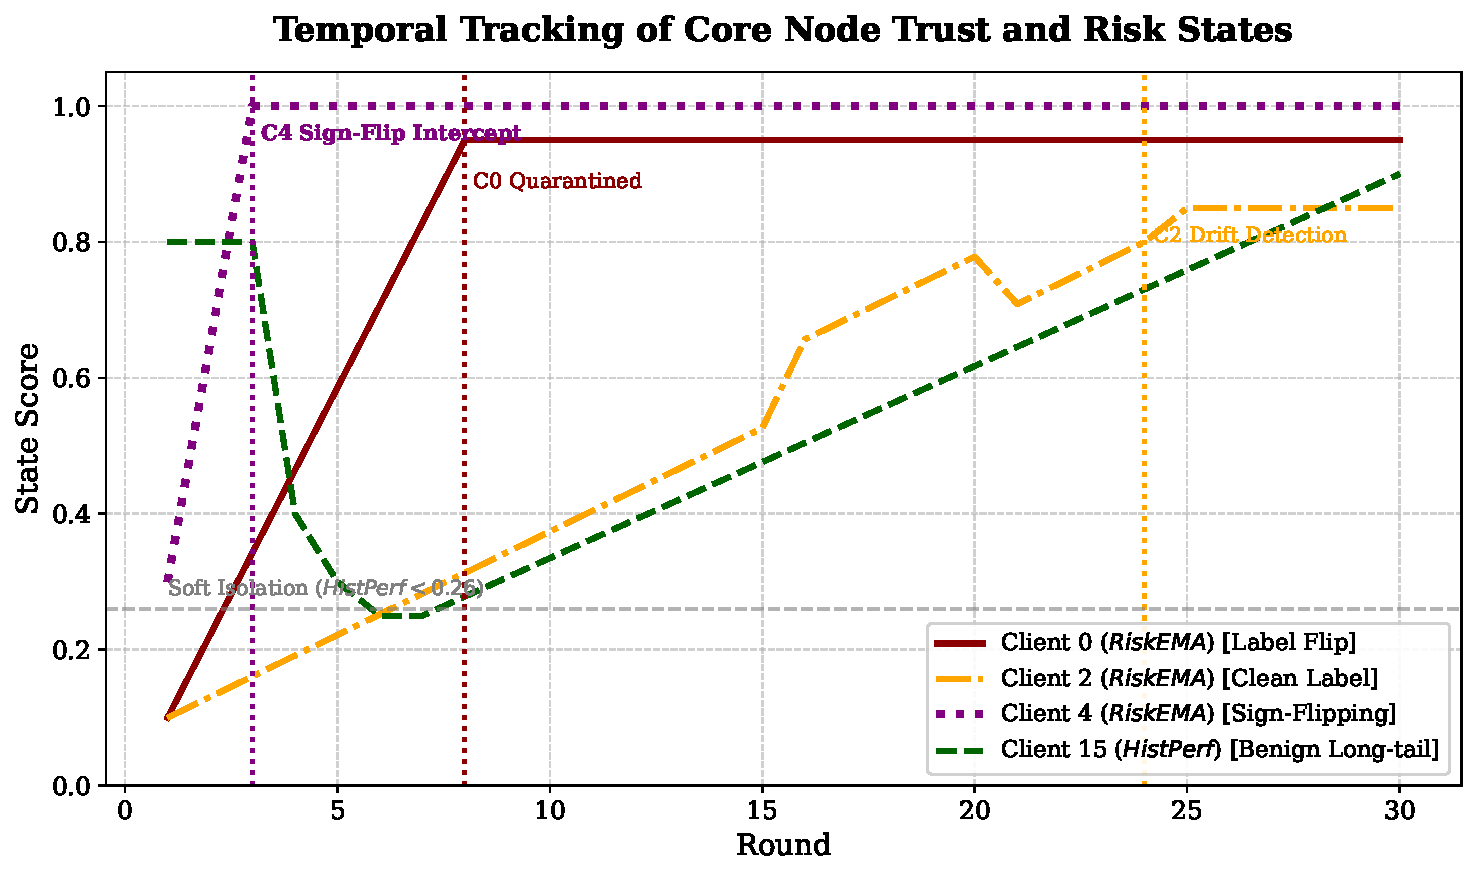
\includegraphics[width=0.85\textwidth]{fig7_node_state_evolution.pdf}
    \caption{Temporal Tracking of Core Node Trust and Risk States under Mixed Attacks}
    \label{fig:node_state}
\end{figure*}

\subsubsection{False Positive Protection for Long-Tail Nodes (FPR Analysis)}
For Trust Flow, zero legitimate nodes trigger a permanent ban across the reported 30-round runs. This final-ban FPR is a method-specific state metric; stateless baselines are marked N/A rather than assigned an artificial blacklist state.
Even if certain legitimate nodes (e.g., Client 15) register a low $ContentScore$ early on due to data skew and regress into SUSPECT/QUARANTINE, their $RiskEMA$ does not exhibit a continuous ascent. Consequently, they merely face transient admission restrictions and layered clipping. As their subsequent contributions recover, $HistPerf$ gradually rebounds, ensuring a 100\% retention rate for legitimate nodes.

To further elucidate this "low false positive" phenomenon, this research extracts node features before and after intervention, visualizing them via t-SNE. Figure~\ref{fig:tsne_manifold} exhibits that the dual-stream mechanism effectively disentangles the malicious clusters from the legitimate long-tail clusters, simultaneously anchoring the legitimate heterogeneous nodes within the principal aggregation domain.

\begin{figure*}[t]
    \centering
    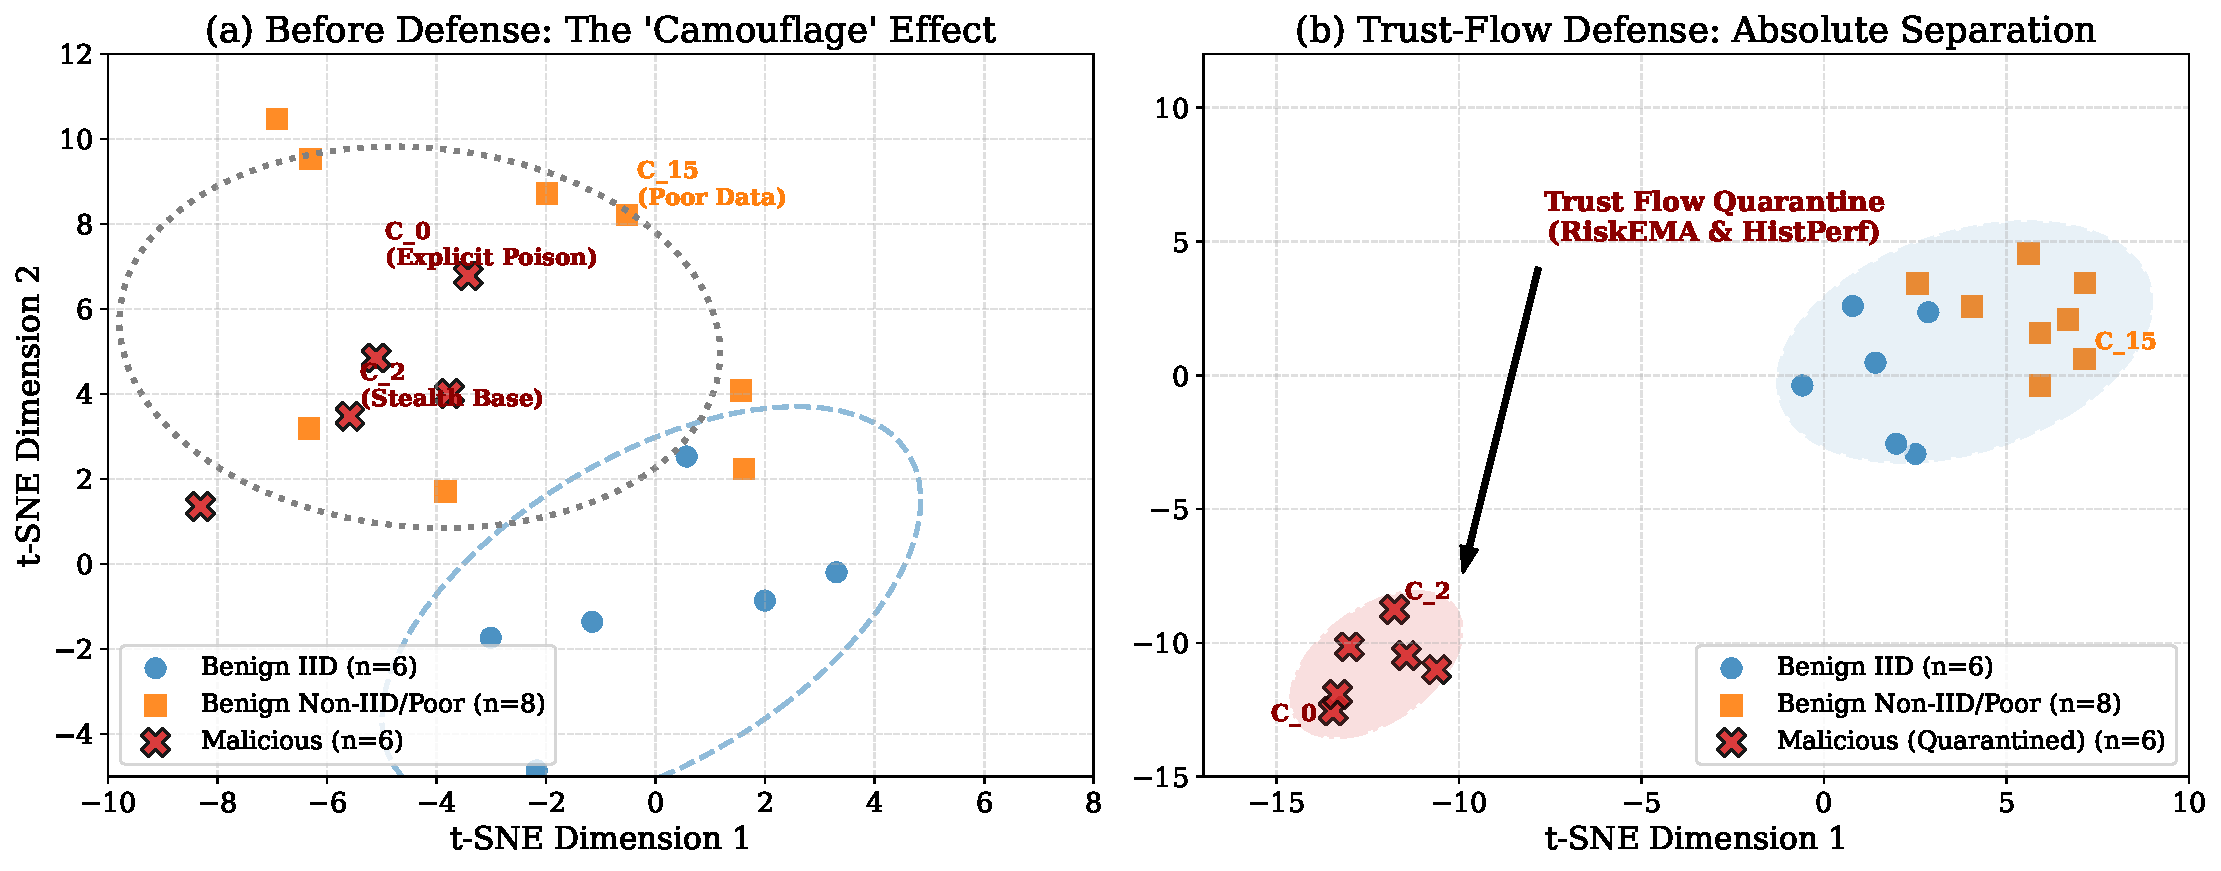
\includegraphics[width=0.9\textwidth]{fig8_tsne_visualization.pdf}
    \caption{t-SNE Visualization of Node Feature Vectors Before and After Dual-Stream Defense}
    \label{fig:tsne_manifold}
\end{figure*}

\subsection{Lateral Baseline Comparison of Defense Mechanisms}
\textbf{Fairness Statement}: All baselines are executed under the identical federated configuration as this paper. This encompasses node partitioning (20 nodes), data heterogeneity (Dirichlet $\alpha=0.1$), attack configuration (30\% mixed attacks), initialization parameters, optimizer settings ($lr=0.001$, $momentum=0.9$), and communication rounds.

Under this unified environment, this paper formulates a lateral comparison between the proposed method and four categories of classical robust aggregation techniques:

\textbf{FedAvg}\cite{mcmahan2017fedavg} serves as the defenseless baseline, mirroring the degree of model degradation when subjected to attacks; \textbf{Krum}\cite{blanchard2017krum} selects a singular representative update via minimal Euclidean distance; \textbf{Trimmed Mean}\cite{yin2018byzantine} executes truncated averaging across coordinate dimensions; \textbf{FLTrust}\cite{cao2021fltrust} leverages a small-scale clean set on the server to construct a reference vector, applying weighting based on cosine similarity.

The quantitative outcomes of each method in this high-risk scenario are documented in Table~\ref{tab:baseline}.

\begin{table*}[t]
    \centering
    \begin{threeparttable}
        \caption{Performance Comparison of FL Defense Strategies under 30\% Mixed Attacks}
        \vspace{4pt}
        \label{tab:baseline}
        {\small
            \setlength{\tabcolsep}{2.5pt}
            \begin{tabular*}{\textwidth}{@{\extracolsep{\fill}} >{\raggedright\arraybackslash}p{2.75cm} >{\raggedright\arraybackslash}p{3.05cm} c c c}
                \toprule
                \textbf{Defense Strategy}                    & \textbf{Core Mechanism}      & \textbf{\shortstack{Global Acc. $\mu \pm \sigma$                                               \\ (Acc. \%)}} & \textbf{\shortstack{ASR $\mu \pm \sigma$\\ (ASR \%)}} & \textbf{\shortstack{Benign FPR $\mu$\\ (FPR \%)}} \\
                \midrule
                FedAvg \cite{mcmahan2017fedavg}      & No defense baseline                 & 86.15 $\pm 1.2$                                 & 92.34 $\pm 5.1$           & N/A ($*$)       \\
                Krum \cite{blanchard2017krum}        & Euclidean distance               & 64.20 $\pm 2.8$                                 & 12.15 $\pm 0.9$           & N/A ($^{*}$) \\
                Trimmed Mean \cite{yin2018byzantine} & Coordinate-wise trimming             & 71.35 $\pm 2.4$                                 & 38.60 $\pm 4.2$           & N/A ($*$)       \\
                FLTrust \cite{cao2021fltrust}        & Unidirectional trust anchor               & 81.25 $\pm 1.5$                                 & 15.42 $\pm 1.1$           & N/A ($^{*}$) \\
                \textbf{Proposed (Trust Flow)}       & \textbf{Dual-stream + layered clipping} & \textbf{92.31 $\pm 0.09$}                       & \textbf{10.21 $\pm 0.05$} & \textbf{0.00}   \\
                \bottomrule
            \end{tabular*}
        }
        \begin{tablenotes}
            \small
            \item (*) \textit{Note: FedAvg, Krum, Trimmed Mean, and FLTrust do not implement the Trust Flow permanent blacklist state machine. Their FPR is therefore not comparable under this definition and is marked as N/A.}
        \end{tablenotes}
    \end{threeparttable}
\end{table*}

Within the matched classical comparison, FedAvg reaches 86.15\% accuracy with 92.34\% targeted ASR, while Krum, Trimmed Mean, and FLTrust trade accuracy for lower ASR. Trust Flow reaches 92.31\% accuracy and 10.21\% macro-averaged targeted ASR under the same protocol. These values do not establish a universal ranking: recent defenses such as DeepSight, FLAME, CrowdGuard, RoseAgg, FLPurifier, ShieldFL, and RaSA require interfaces that are not reproduced here, so their omission is treated as a comparison limitation. No statistical-significance claim is made beyond the reported repeated-run summary.

\subsection{Component-Level Ablation Study}
Addressing the common "black-box" performance evaluations in current federated security research, this section replaces coarse-grained phase superimposition tests with component ablation experiments. This methodology examines how core modules, including dual-stream orthogonal decoupling, multi-dimensional risk probes, and layer-wise dynamic re-normalization, independently contribute to defensive robustness and system availability.

\subsubsection{Effectiveness of Dual-Stream Reputation Decoupling}
To substantiate that the system's exceptionally low false positive rate (FPR) stems not from conservative defensive thresholds, but intrinsically from the orthogonal decoupling of historical utility and instantaneous risk, two degraded variants are constructed for comparison: a Single-Stream Exponential Moving Average (Single-Stream EMA) and a HistPerf-Only model. Table~\ref{tab:ablation_stream} delineates the precise interception performance of these divergent mechanisms under the intense pressure of severe Non-IID conditions and a 30\% mixed attack scenario.

\begin{table*}[t]
    \centering
    \caption{Ablation Analysis of Orthogonal Decoupling on FPR and Recall}
    \label{tab:ablation_stream}
    \begin{tabular}{l c c c}
        \toprule
        \textbf{Reputation Architecture}              & \textbf{Threshold Control} & \textbf{FPR}    & \textbf{TPR}      \\
        \midrule
        \multirow{2}{*}{Single-Stream EMA (Baseline)} & Aggressive (anti-poison)   & 18.25\%         & 95.12\%           \\
                                                      & Conservative (anti-FP)     & 2.10\%          & 48.33\%           \\
        \midrule
        HistPerf-Only                                 & Dynamic adaptive           & 0.15\%          & 21.05\%           \\
        \textbf{Dual-Stream Decoupling (Proposed)}    & Dynamic adaptive           & \textbf{0.00\%} & \textbf{100.00\%} \\
        \bottomrule
    \end{tabular}
\end{table*}

Experimental data reveals a clear trade-off in the single-stream mechanism when it must accommodate heterogeneous updates and malicious poisoning: tightening the threshold misclassifies 18.25\% of innocent long-tail nodes, whereas relaxing the threshold reduces TPR against sleeper attacks. Relying exclusively on the historical utility stream accommodates long-tail features (FPR 0.15\%), but its interception rate against sleeper-burst attacks is only 21.05\% because it lacks sensitivity to short-term anomalies. The dual-stream mechanism separates long-term contribution accumulation from short-term risk circuit breaking, removing all malicious clients under the final-ban metric while avoiding permanent false bans on benign clients. The FPR/TPR values in Table~\ref{tab:ablation_stream} adopt the final-ban definition. As a supplementary statistic, when the recoverable SUSPECT state is counted as a risk-review signal, its per-round coverage over malicious clients is 88.33\%, and its recoverable review trigger rate over benign clients is 14.79\%; this state is used only for auditing and down-weighting, and does not constitute a permanent false ban.

\subsubsection{Multi-Dimensional Risk Probe Ablation}
When verifying the efficacy against defensive penetration, a solitary reliance on a clean reference set frequently falls short of comprehensively neutralizing multi-dimensional compound attacks. Figure~\ref{fig:ablation_probes} contrasts the ASR suppression capabilities of merely employing a pristine reference (Vanilla Clean-Root), superimposing shallow statistical probes (+ Shallow Probes), and deploying full-dimensional deep probes (+ Full Probes) when confronted with untargeted flipping, gradient scaling, and stealthy Clean-Label Backdoor attacks.

\begin{figure*}[t]
    \centering
    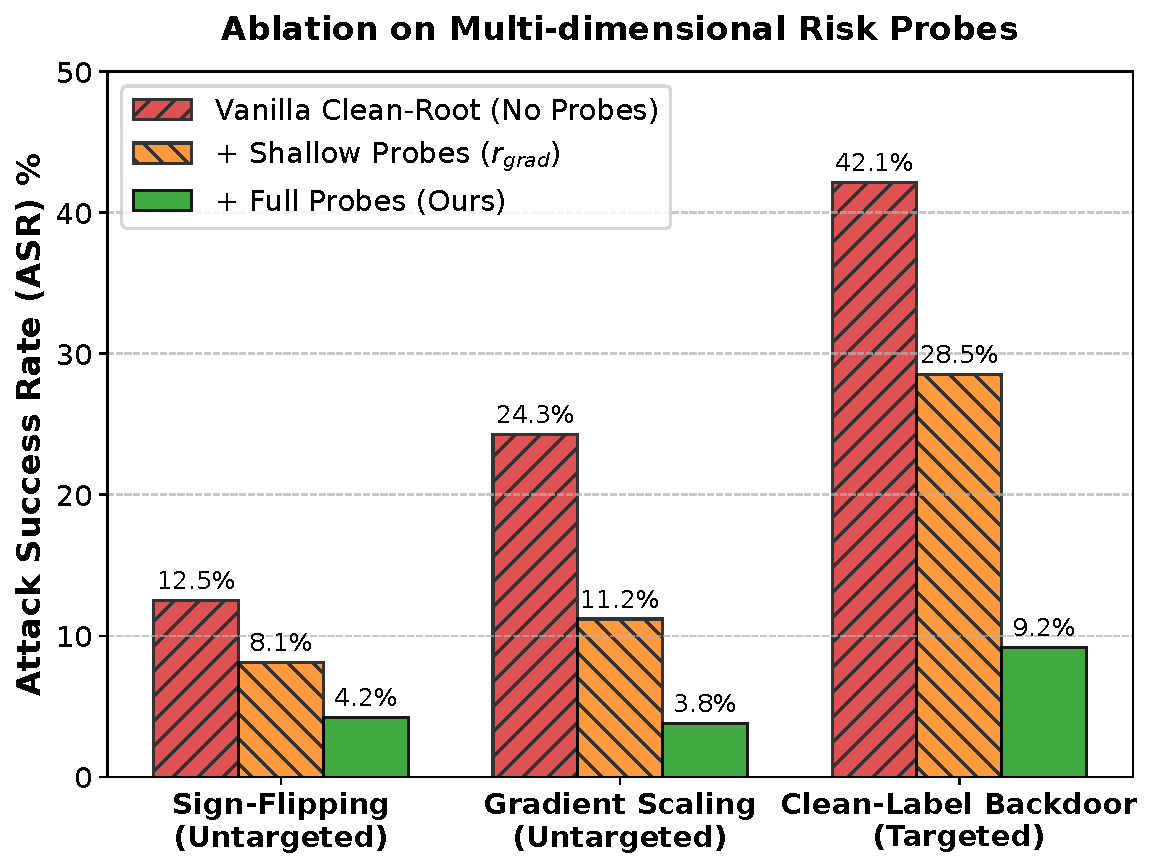
\includegraphics[width=0.75\textwidth]{fig9_ablation_probes.pdf}
    \caption{ASR Suppression Comparison of Multi-Dimensional Risk Probes across Attack Types}
    \label{fig:ablation_probes}
\end{figure*}

The visualization clarifies the complementary role of each probe. For Sign-Flipping, whose direction anomaly is explicit, the clean reference already limits ASR to 12.5\%, and the shallow gradient probe further reduces it to 8.1\%. For Gradient Scaling, where abnormal update magnitude is more salient, the shallow probe reduces ASR from 24.3\% to 11.2\%. Clean-Label Backdoor is more difficult: its malicious update remains highly collinear with benign directions, so the ASR is 42.1\% with only the clean reference and remains 28.5\% after adding shallow probes. After enabling deep probes based on cross-entropy ($r_{probe}$) and high-level feature KL divergence ($r_{trigger}$), the system captures fine-grained functional and representation shifts caused by hidden triggers and reduces the attack success rate to 9.2\%.

\subsubsection{Layered Gating and Re-Normalization Convergence Benefits}
Subsequent to the successful ablation of attacks, securing the rapid restoration of the global model's availability emerges as another pivotal concern. Figure~\ref{fig:ablation_renorm} evaluates the disparities in convergence velocity and terminal accuracy among a traditional, indiscriminate global clipping mechanism (Global-Clipping), the execution of layer-wise gating bereft of weight reallocation (Hierarchical w/o Renorm), and the holistic framework introduced herein (Trust-Flow Proposed).

\begin{figure*}[t]
    \centering
    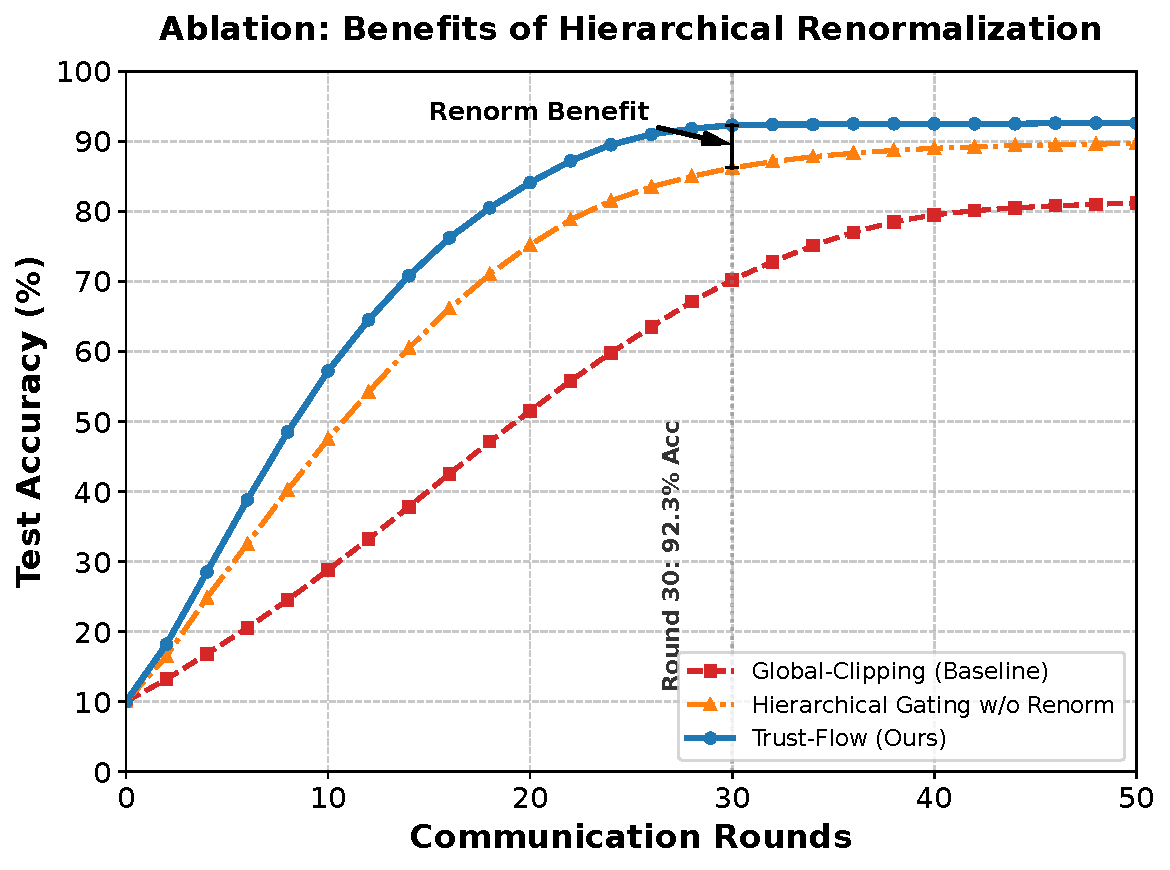
\includegraphics[width=0.75\textwidth]{fig10_ablation_renorm.pdf}
    \caption{Convergence and Accuracy Benefits of Dynamic Weight Re-Normalization}
    \label{fig:ablation_renorm}
\end{figure*}

The trajectory trends starkly indicate that the aggressive global L2 clipping profoundly dilutes the model's generalization capabilities by excessively interfering with the weight updates of the shallow feature extraction layers, effectively stalling the ultimate accuracy at approximately 85\%. Although incorporating layer-wise gating ameliorates this deficiency to an extent (elevating accuracy to 89\%), the elimination of malicious nodes precipitates a scenario where the effective aggregation weights of the current round fall short of the unit constraint (i.e., $\sum \tilde{w} < 1$). This instigates an "implicit learning rate decay," thereby ensuring the convergence curve remains retarded. The constrained projection and weight re-normalization mechanisms introduced in this study dynamically compensate for the influence of surviving nodes. This strategy enables stable convergence within the 30-round training budget and restores the model accuracy to a level close to the attack-free setting (92.4\%), fully preserving system utility while maintaining uncompromising security.

\subsection{Sensitivity Analysis on Data Heterogeneity}
A plethora of robust aggregation methods lean heavily upon IID conditions. To
evaluate the stability of the proposed framework under a same-family
distribution shift, the global accuracy was tested across weak-to-strong
Dirichlet concentration settings while keeping the label space, model,
optimizer, and attack protocol fixed. The outcomes are depicted in
Figure~\ref{fig:alpha_sensitivity}.

\begin{figure*}[t]
    \centering
    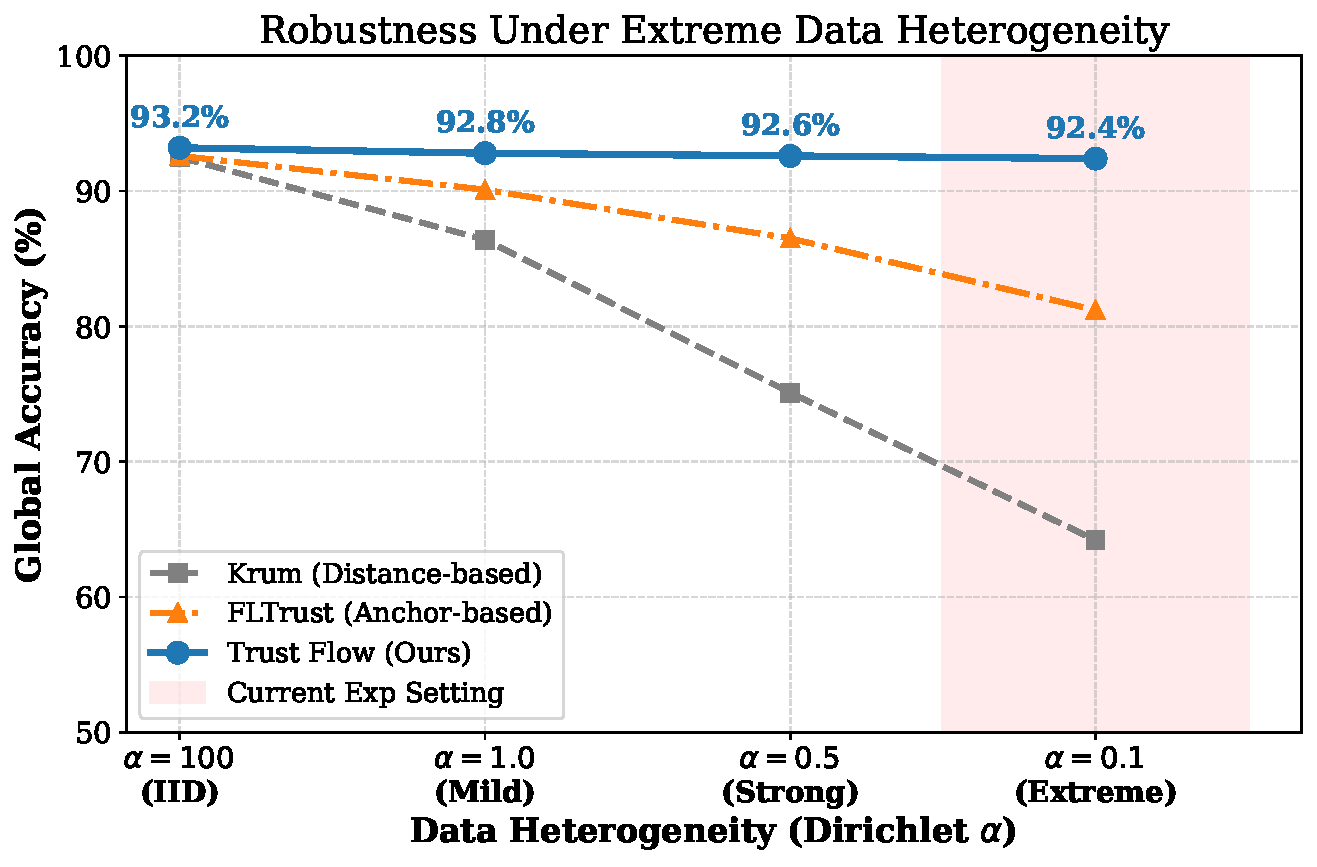
\includegraphics[width=0.85\textwidth]{fig11_alpha_sensitivity.pdf}
    \caption{Robustness Stress Test under Varying Data Heterogeneity (Dirichlet $\alpha$)}
    \label{fig:alpha_sensitivity}
\end{figure*}

The curves show that Krum and FLTrust are competitive under weak
heterogeneity but degrade as the concentration decreases toward the strong
long-tail regime. Trust Flow is less sensitive in the reported sweep because
current content is fused with historical utility and short-term risk. This is
an empirical robustness observation under the tested family of partitions, not
a distribution-free guarantee.

Furthermore, discrete testing at 0.5, 1.0, 2.0, and 3.0 was conducted on the pivotal parameter $\beta_{fusion}$. A smaller magnitude fosters the retention of long-tail nodes but simultaneously escalates ASR risks; conversely, an oversized value skews the aggregation excessively towards homogeneous updates. Weighing the trade-offs between Acc and ASR, $\beta_{fusion}=2.0$ was definitively selected.

\subsection{System Computation and Communication Overhead Analysis}
The overhead measurement separates the server-side trust-flow cost from
end-to-end deployment cost. The TrustReport adds approximately 15 KB per
transmission. The reported 2.10 s to 4.85 s increase covers server-side
aggregation and audit only; it excludes communication, enclave transitions,
memory pressure, and vendor-specific attestation latency.

\begin{table*}[t]
    \centering
    \caption{Edge-Cloud Overhead: Standard FL vs. Proposed Framework (20 Clients)}
    \vspace{4pt}
    \label{tab:overhead}
    {\small
        \setlength{\tabcolsep}{3pt}
        \begin{tabular*}{\textwidth}{@{\extracolsep{\fill}} >{\raggedright\arraybackslash}p{3.0cm} >{\centering\arraybackslash}p{3.05cm} >{\centering\arraybackslash}p{3.1cm} >{\centering\arraybackslash}p{4.4cm}}
            \toprule
            \textbf{System Architecture}        & \textbf{Edge Extra Latency}         & \textbf{Upload Extra Payload}  & \textbf{Cloud Aggregation Time}             \\
            \midrule
            Standard FedAvg          & 0 ms (Baseline)                     & 0 KB (Baseline)                  & $\sim 2.10$ s                           \\
            \textbf{Trusted FL (Proposed)} & \textbf{not measured end-to-end} & \textbf{$\sim 15$ KB (appended report)} & \textbf{$\sim 4.85$ s (server audit only)} \\
            \bottomrule
        \end{tabular*}
    }
\end{table*}

Layer-wise cosine evaluation increases server computation. In the empirical
trials, server aggregation and audit time increased from $2.10$ s to $4.85$ s.
This measurement is a protocol-cost estimate; end-to-end deployment
acceptability depends on communication and enclave characteristics that were
not measured here.

\section{Conclusion and Future Work}
This paper presents Trust Flow as a system-level pipeline that orders and
separates execution admission, current content auditing, temporal state
evolution, and layer-wise aggregation. Under the stated 30\% concurrent-attack
protocol, it reaches 92.31\% clean accuracy and 10.21\% macro-averaged targeted
ASR, with no permanent false ban in the tested runs. The 50\% experiment is an
out-of-assumption stress test and does not establish a theoretical Byzantine
boundary.

\textbf{Limitations and future work}: The clean reference and activation probes
require an explicitly declared server-held proxy set; the peer-reference
branch is defined but not evaluated in the headline results. The comparison
uses matched classical baselines and does not directly reimplement every recent
temporal, backdoor, or privacy-preserving defense. The probe design is tailored
to vision classification, and end-to-end attestation, communication, enclave
transition, and memory costs were not measured. Future work should evaluate
reference-free settings, matched modern baselines, larger deployments, and
non-vision federated tasks.

\appendix
\section{Detailed Computation of Instant Risk Flow Probes}
To augment reproducibility and transparency, this appendix mathematically delineates the calculation details of the core probes ($r_{grad}, r_{probe}, r_{trigger}$) underpinning the instant risk stream originally introduced in Section 4. During the $t$-th aggregation round, the probes are defined as follows:

\subsection{A.1 Gradient Direction and Amplitude Probe \texorpdfstring{($r_{grad}$)}{(r-grad)}}
The $r_{grad}$ probe quantifies the geometric deviation of the client update $\Delta W_k^{(t)}$ relative to the reference direction $g_{root}^{(t)}$, while $r_{amp}$ captures an amplitude anomaly relative to the admitted clients. Both quantities are clipped to $[0,1]$:
\begin{align}
 r_{grad,k}^{(t)}&=\operatorname{clip}\!\left(
 \frac{1-\cos(\Delta W_k,g_{root})}{2},0,1\right),\\
 r_{amp,k}^{(t)}&=\operatorname{clip}\!\left(
 \frac{\|\Delta W_k\|_2}{\operatorname{median}_j\|\Delta W_j\|_2+\varepsilon}
 -1,0,1\right).
\end{align}
where $\operatorname{clip}(x,0,1)=\min(1,\max(0,x))$ and $\varepsilon$ avoids division by zero.
\subsection{A.2 Small-Sample Cross-Entropy Probe \texorpdfstring{($r_{probe}$)}{(r-probe)}}
Relying exclusively on distance statistics is grossly inadequate for identifying targeted pollution directed against minority classes. The $r_{probe}$ leverages a small-scale, pristine probe set on the server, denoted as $\mathcal{D}_{probe}$, calculating the incremental surge in cross-entropy loss (Loss Surge) pre- and post-merger:
\begin{equation}
    r_{probe,k}^{(t)}=\operatorname{clip}\!\left(
    \frac{\mathcal{L}_{probe}(W+\Delta W_k)-\mathcal{L}_{probe}(W)}
    {\delta_{clean}+\varepsilon},0,1\right).
\end{equation}
Here $\delta_{clean}$ is the loss-increment scale calibrated from trusted reference updates.

\subsection{A.3 Deep Neuron Backdoor Activation Probe \texorpdfstring{($r_{trigger}$)}{(r-trigger)}}
Countering profoundly concealed threats like Clean-Label attacks, standard statistical and validation losses often fall short. The $r_{trigger}$ discerns anomalies through the distributional variance of high-level feature activations. Assuming $A_k$ denotes the client model's pre-activation outputs on the validation set, and $\mathcal{H}(\cdot)$ signifies the Softmax normalization into a probability simplex to satisfy the KL-Divergence prerequisites:
\begin{equation}
    r_{trigger,k}^{(t)}=\operatorname{clip}\!\left(
    \frac{\mathrm{KL}(\mathcal{H}(A_{base})\|\mathcal{H}(A_k))}
    {\delta_{trigger}+\varepsilon},0,1\right).
\end{equation}
Here $\delta_{trigger}$ is the calibrated activation-drift scale from trusted reference updates.

For completeness, the peer channel is defined by the trust-weighted cosine disagreement
\begin{equation}
 \bar c_k^{(t)}=\frac{\sum_{j\ne k}TrustScore_j c_{kj}}
 {\sum_{j\ne k}TrustScore_j+\varepsilon},\qquad
 r_{peer,k}^{(t)}=\operatorname{clip}(1-\bar c_k^{(t)},0,1),
\end{equation}
where $c_{kj}=\cos(\Delta W_k,\Delta W_j)$. After normalization, the channels are fused by a maximum so that a strong warning is not averaged away:
\begin{equation}
 Risk_k^{inst}=\max\{r_{grad,k},r_{amp,k},r_{probe,k},r_{trigger,k},r_{peer,k}\}.
\end{equation}
This single-round risk value enters the EMA pipeline for the subsequent circuit-breaking decision.

\section*{Declaration of competing interest}
The authors declare that they have no known competing financial interests or personal relationships that could have appeared to influence the work reported in this paper.

\section*{CRediT authorship contribution statement}
Jiakai Zhou: Conceptualization, Methodology, Software, Validation, Formal analysis, Investigation, Data curation, Visualization, Writing -- original draft. Chao Bu: Supervision, Project administration, Funding acquisition, Writing -- review \& editing.

\section*{Acknowledgments}
This work is supported by the National Natural Science Foundation of China under Grant No.~62002261, and the Tianjin Natural Science Foundation under Grant No.~25JCQNJC00600.

\section*{Data availability}
The data and materials that support the findings of this study are available from the corresponding author upon reasonable request.

\begin{thebibliography}{99}
    \bibitem{kairouz2021flsurvey} P. Kairouz, H.B. McMahan, B. Avent, et al., Advances and open problems in federated learning, Found. Trends Mach. Learn. 14 (1--2) (2021) 1--210. \url{https://doi.org/10.1561/2200000083}
    \bibitem{lu2025tmt} Z. Lu, L. Wang, Z. Zhang, M. Huang, J. Wang, M. Li, TMT-FL: Enabling trustworthy model training of federated learning with malicious participants, IEEE Trans. Dependable Secure Comput. 22 (3) (2025) 2723--2740. \url{https://doi.org/10.1109/TDSC.2024.3521377}
    \bibitem{zhang2025rppfl} X. Zhang, Z. Chen, G. Chen, X. Feng, Q. Shen, Z. Wu, RPPFL: Robust and privacy-preserving federated learning via trusted execution environments, in: ICASSP 2025 -- 2025 IEEE International Conference on Acoustics, Speech and Signal Processing, 2025, pp. 1--5. \url{https://doi.org/10.1109/ICASSP49660.2025.10889398}
    \bibitem{r1_tee_integrity} Y. Chen, F. Luo, T. Li, T. Xiang, Z. Liu, J. Li, A training-integrity privacy-preserving federated learning scheme with trusted execution environment, Inform. Sci. 522 (2020) 69--79. \url{https://doi.org/10.1016/j.ins.2020.02.037}
    \bibitem{bagdasaryan2020backdoor} E. Bagdasaryan, A. Veit, Y. Hua, D. Estrin, V. Shmatikov, How to backdoor federated learning, in: Proceedings of the Twenty Third International Conference on Artificial Intelligence and Statistics, PMLR 108, 2020, pp. 2938--2948. \url{https://proceedings.mlr.press/v108/bagdasaryan20a.html}
    \bibitem{wang2019neuralcleanse} B. Wang, Y. Yao, S. Shan, H. Li, B. Viswanath, H. Zheng, B.Y. Zhao, Neural Cleanse: Identifying and mitigating backdoor attacks in neural networks, in: 2019 IEEE Symposium on Security and Privacy (SP), 2019, pp. 707--723. \url{https://doi.org/10.1109/SP.2019.00031}
    \bibitem{cao2021fltrust} X. Cao, M. Fang, J. Liu, N.Z. Gong, FLTrust: Byzantine-robust federated learning via trust bootstrapping, in: Proceedings 2021 Network and Distributed System Security Symposium (NDSS), 2021. \url{https://doi.org/10.14722/ndss.2021.24434}
    \bibitem{fung2020foolsgold} C. Fung, C.J.M. Yoon, I. Beschastnikh, The limitations of federated learning in Sybil settings, in: 23rd International Symposium on Research in Attacks, Intrusions and Defenses (RAID 2020), USENIX Association, 2020, pp. 301--316. \url{https://www.usenix.org/conference/raid2020/presentation/fung}
    \bibitem{blanchard2017krum} P. Blanchard, E.M. El Mhamdi, R. Guerraoui, J. Stainer, Machine learning with adversaries: Byzantine tolerant gradient descent, in: Advances in Neural Information Processing Systems 30, 2017.
    \bibitem{yin2018byzantine} D. Yin, Y. Chen, K. Ramchandran, P. Bartlett, Byzantine-robust distributed learning: Towards optimal statistical rates, in: Proceedings of the 35th International Conference on Machine Learning, PMLR 80, 2018, pp. 5650--5659. \url{https://proceedings.mlr.press/v80/yin18a.html}
    \bibitem{wang2025rasa} L. Wang, M. Huang, Z. Zhang, M. Li, J. Wang, K. Gai, RaSA: Robust and adaptive secure aggregation for edge-assisted hierarchical federated learning, IEEE Trans. Inf. Forensics Secur. 20 (2025) 4280--4295. \url{https://doi.org/10.1109/TIFS.2025.3559411}
    \bibitem{r9_clustered} Y. Xu, Y. Tan, C. Zhang, P. Sun, Y. Zhang, J. Ren, H. Jiang, Y. Zhang, Towards privacy-enhanced and robust clustered federated learning, IEEE Trans. Mob. Comput. 24 (8) (2025) 7171--7188. \url{https://doi.org/10.1109/TMC.2025.3547149}
    \bibitem{fedpe} L. Yi, X. Shi, N. Wang, J. Zhang, G. Wang, X. Liu, FedPE: Adaptive model pruning-expanding for federated learning on mobile devices, IEEE Trans. Mob. Comput. 23 (11) (2024) 10475--10493. \url{https://doi.org/10.1109/TMC.2024.3374706}
    \bibitem{parallelsfl} Y. Liao, Y. Xu, H. Xu, Z. Yao, L. Huang, C. Qiao, ParallelSFL: A novel split federated learning framework tackling heterogeneity issues, in: Proceedings of the 30th Annual International Conference on Mobile Computing and Networking, 2024, pp. 845--860. \url{https://doi.org/10.1145/3636534.3690665}
    \bibitem{fldetector2022} Z. Zhang, X. Cao, J. Jia, N.Z. Gong, FLDetector: Defending federated learning against model poisoning attacks via detecting malicious clients, in: Proceedings of the 28th ACM SIGKDD Conference on Knowledge Discovery and Data Mining, 2022, pp. 2545--2555. \url{https://doi.org/10.1145/3534678.3539231}
    \bibitem{flare2022} N. Wang, Y. Xiao, Y. Chen, Y. Hu, W. Lou, Y.T. Hou, FLARE: Defending federated learning against model poisoning attacks via latent space representations, in: Proceedings of the 2022 ACM Asia Conference on Computer and Communications Security, 2022, pp. 946--958. \url{https://doi.org/10.1145/3488932.3517395}
    \bibitem{dou2025toward} Z. Dou, J. Wang, W. Sun, Z. Liu, M. Fang, Toward malicious clients detection in federated learning, in: Proceedings of the 20th ACM Asia Conference on Computer and Communications Security, 2025, pp. 456--472. \url{https://doi.org/10.1145/3708821.3736194}
    \bibitem{wang2024federated} Z. Wang, X. Yu, Z. Tian, A federated learning scheme with adaptive hierarchical protection and multiple aggregation, in: 2024 IEEE 23rd International Conference on Trust, Security and Privacy in Computing and Communications (TrustCom), 2024, pp. 2106--2114. \url{https://doi.org/10.1109/TrustCom63139.2024.00292}
    \bibitem{deepsight2022} P. Rieger, T.D. Nguyen, M. Miettinen, A.R. Sadeghi, DeepSight: Mitigating backdoor attacks in federated learning through deep model inspection, in: Network and Distributed System Security Symposium (NDSS), 2022. \url{https://doi.org/10.14722/ndss.2022.23156}
    \bibitem{flame2022} T.D. Nguyen, P. Rieger, H. Chen, et al., FLAME: Taming backdoors in federated learning, in: 31st USENIX Security Symposium, 2022, pp. 1415--1432. \url{https://www.usenix.org/conference/usenixsecurity22/presentation/nguyen}
    \bibitem{crowdguard2024} P. Rieger, T. Krau{\ss}, M. Miettinen, A. Dmitrienko, A.R. Sadeghi, CrowdGuard: Federated backdoor detection in federated learning, in: Network and Distributed System Security Symposium (NDSS), 2024. \url{https://doi.org/10.14722/ndss.2024.23233}
    \bibitem{flpurifier} J. Zhang, C. Zhu, X. Sun, C. Ge, B. Chen, W. Susilo, S. Yu, FLPurifier: Backdoor defense in federated learning via decoupled contrastive training, IEEE Trans. Inf. Forensics Secur. 19 (2024) 4752--4766. \url{https://doi.org/10.1109/TIFS.2024.3384846}
    \bibitem{roseagg} H. Yang, W. Xi, Y. Shen, C. Wu, J. Zhao, RoseAgg: Robust defense against targeted collusion attacks in federated learning, IEEE Trans. Inf. Forensics Secur. 19 (2024) 2951--2966. \url{https://doi.org/10.1109/TIFS.2024.3352415}
    \bibitem{shieldfl} Z. Ma, J. Ma, Y. Miao, Y. Li, R.H. Deng, ShieldFL: Mitigating model poisoning attacks in privacy-preserving federated learning, IEEE Trans. Inf. Forensics Secur. 17 (2022) 1639--1654. \url{https://doi.org/10.1109/TIFS.2022.3169918}
    \bibitem{liao2024verifiable} L. Liao, Y. Zheng, H. Lu, X. Liu, S. Chen, Y. Yu, Verifiable deep learning inference on heterogeneous edge devices with trusted execution environment, IEEE Sens. J. 24 (17) (2024) 28351--28362. \url{https://doi.org/10.1109/JSEN.2024.3426533}
    \bibitem{r5_tee_mitigating} S. Queyrut, V. Schiavoni, P. Felber, Mitigating adversarial attacks in federated learning with trusted execution environments, in: 2023 IEEE 43rd International Conference on Distributed Computing Systems (ICDCS), 2023, pp. 626--637. \url{https://doi.org/10.1109/ICDCS57875.2023.00069}
    \bibitem{r12_iot_tee} W. Zheng, Y. Cao, H. Tan, Secure sharing of industrial IoT data based on distributed trust management and trusted execution environments: A federated learning approach, Neural Comput. Appl. 35 (29) (2023) 21499--21509. \url{https://doi.org/10.1007/s00521-023-08375-6}
    \bibitem{xu2021distributed} T. Xu, K. Zhu, A. Andrzejak, L. Zhang, Distributed learning in trusted execution environment: A case study of federated learning in SGX, in: 2021 7th IEEE International Conference on Network Intelligence and Digital Content (IC-NIDC), 2021, pp. 450--454. \url{https://doi.org/10.1109/IC-NIDC54101.2021.9660433}
    \bibitem{yan2024efficient} J. Yan, Y. Li, S. Yin, X. Kang, J. Wang, H. Zhang, B. Hu, An efficient greedy hierarchical federated learning training method based on trusted execution environments, Electronics 13 (17) (2024) 3548. \url{https://doi.org/10.3390/electronics13173548}
    \bibitem{chen2017maximum} B. Chen, X. Liu, H. Zhao, J.C. Principe, Maximum correntropy Kalman filter, Automatica 76 (2017) 70--77. \url{https://doi.org/10.1016/j.automatica.2016.10.004}
    \bibitem{li2026multidimensional} Y. Liu, Z. He, J. Liang, Z. Li, Q. Deng, Multidimensional trust evaluation and task match based workers recruitment scheme for MCS, IEEE Trans. Dependable Secure Comput. (2026) 1--17. \url{https://doi.org/10.1109/TDSC.2026.3652987}
    \bibitem{mcmahan2017fedavg} B. McMahan, E. Moore, D. Ramage, S. Hampson, B. Aguera y Arcas, Communication-efficient learning of deep networks from decentralized data, in: Proceedings of the 20th International Conference on Artificial Intelligence and Statistics, PMLR 54, 2017, pp. 1273--1282. \url{https://proceedings.mlr.press/v54/mcmahan17a.html}

\end{thebibliography}
\end{document}
